\documentclass[11pt,letterpaper,twocolumn]{article}
\usepackage[utf8]{inputenc}
\usepackage[T1]{fontenc}
\usepackage{graphicx}
\usepackage{amsmath}
\usepackage{amssymb}
\usepackage{geometry}
\usepackage{tikz}
\usepackage{xcolor}
\usepackage{stfloats}
\usepackage{flushend}
\usetikzlibrary{shapes.geometric, arrows.meta, positioning, fit, backgrounds, calc}

\geometry{margin=0.65in, columnsep=16pt}

% Allow more floats per page and tighter placement
\setcounter{topnumber}{4}
\setcounter{bottomnumber}{3}
\setcounter{totalnumber}{6}
\renewcommand{\topfraction}{0.90}
\renewcommand{\bottomfraction}{0.70}
\renewcommand{\textfraction}{0.07}
\renewcommand{\floatpagefraction}{0.85}

% Tight float spacing
\setlength{\textfloatsep}{7pt plus 2pt minus 2pt}
\setlength{\floatsep}{5pt plus 1pt minus 1pt}
\setlength{\abovecaptionskip}{3pt}
\setlength{\belowcaptionskip}{1pt}

% --- TikZ styles ---
\tikzset{
	block/.style={rectangle, rounded corners=3pt, draw=black!70, fill=blue!12,
		text width=1.55cm, align=center, minimum height=0.75cm, font=\tiny},
	wideblock/.style={rectangle, rounded corners=3pt, draw=black!70, fill=blue!12,
		text width=2.2cm, align=center, minimum height=0.75cm, font=\tiny},
	datablock/.style={rectangle, rounded corners=3pt, draw=black!60, fill=green!12,
		text width=1.55cm, align=center, minimum height=0.7cm, font=\tiny},
	outblock/.style={rectangle, rounded corners=3pt, draw=black!60, fill=orange!15,
		text width=1.55cm, align=center, minimum height=0.7cm, font=\tiny},
	arrow/.style={-{Stealth[length=4pt]}, thick},
	dasharrow/.style={-{Stealth[length=4pt]}, thick, dashed},
	grouplabel/.style={font=\bfseries\tiny, align=center},
	% CDA diagram styles (wider nodes)
	cdablock/.style={rectangle, rounded corners=3pt, draw=black!60, fill=green!12,
		text width=2.3cm, align=center, minimum height=0.8cm, font=\tiny},
	cdaswap/.style={rectangle, rounded corners=3pt, draw=black!70, fill=yellow!25,
		text width=1.5cm, align=center, minimum height=0.8cm, font=\tiny},
	cdaout/.style={rectangle, rounded corners=3pt, draw=black!60, fill=orange!15,
		text width=2.3cm, align=center, minimum height=0.7cm, font=\tiny},
	cdagreen/.style={rectangle, rounded corners=3pt, draw=black!60, fill=green!12,
		text width=2.3cm, align=center, minimum height=0.7cm, font=\tiny},
	cdared/.style={rectangle, rounded corners=3pt, draw=black!60, fill=red!12,
		text width=2.3cm, align=center, minimum height=0.7cm, font=\tiny},
	cdacombined/.style={rectangle, rounded corners=3pt, draw=black!70, fill=purple!15,
		text width=1.8cm, align=center, minimum height=0.7cm, font=\tiny},
	% Compact vertical flowchart styles
	cblock/.style={rectangle, rounded corners=3pt, draw=black!70, fill=blue!12,
		text width=3.6cm, align=center, minimum height=0.8cm, font=\footnotesize},
	cwideblock/.style={rectangle, rounded corners=3pt, draw=black!70, fill=blue!12,
		text width=3.6cm, align=center, minimum height=0.8cm, font=\footnotesize},
	cdatablock/.style={rectangle, rounded corners=3pt, draw=black!60, fill=green!12,
		text width=3.6cm, align=center, minimum height=0.75cm, font=\footnotesize},
	coutblock/.style={rectangle, rounded corners=3pt, draw=black!60, fill=orange!15,
		text width=3.6cm, align=center, minimum height=0.75cm, font=\footnotesize},
}

\title{\textbf{Comprehensive Project Report:\\
		BERT Pre-training and Bias-in-Bios Mitigation}}
\author{Townsend Southard Pantano, Omar Camara}
\date{\today}

\begin{document}
	
	\twocolumn[{%
		\maketitle
		\begin{@twocolumnfalse}
			\begin{abstract}
				This document serves as a comprehensive visual and analytical record of the project.
				It covers the pre-training of a 128M parameter BERT model, the exploratory analysis
				of the Bias-in-Bios dataset, and the comparative evaluation of biased vs.\ debiased
				fine-tuning strategies. We include all 30 metric visualizations generated during the
				project lifecycle.
			\end{abstract}
			\vspace{0.4em}
		\end{@twocolumnfalse}
	}]
	
	% ======================================================================
	\section{Introduction}
	% ======================================================================
	This project investigates the lifecycle of gender bias in NLP models. By training a model
	from scratch and then fine-tuning it under different constraints, we identify how linguistic
	representations can both inherit and mitigate societal disparities.
	
	\subsection{Overall Training Workflow}
	Figure~\ref{fig:workflow} summarises the four-phase pipeline: (1)~pre-training a BERT model
	on general text, (2)~profiling the Bias-in-Bios dataset, (3)~fine-tuning under two
	contrasting regimes, and (4)~comparative evaluation of the resulting models.
	
	\begin{figure}[!htb]
		\centering
		\resizebox{\linewidth}{!}{%
			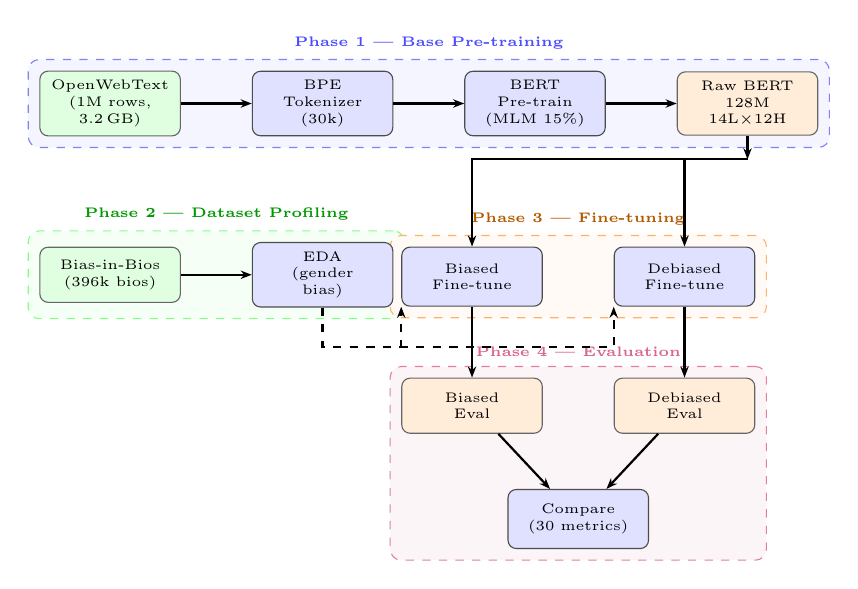
\begin{tikzpicture}[node distance=0.6cm and 0.9cm]
				% Phase 1
				\node[datablock] (owt)  {OpenWebText\\(1M rows,\\3.2\,GB)};
				\node[block, right=of owt] (tok)  {BPE\\Tokenizer\\(30k)};
				\node[block, right=of tok] (bert) {BERT\\Pre-train\\(MLM 15\%)};
				\node[outblock, right=of bert] (rawbert) {Raw BERT\\128M\\14L$\times$12H};
				\draw[arrow](owt)--(tok);\draw[arrow](tok)--(bert);\draw[arrow](bert)--(rawbert);
				\begin{scope}[on background layer]
					\node[draw=blue!50,dashed,rounded corners,inner sep=4pt,
					fit=(owt)(tok)(bert)(rawbert),fill=blue!4,
					label={[grouplabel,blue!70]above:Phase 1 — Base Pre-training}]{};
				\end{scope}
				% Phase 2
				\node[datablock,below=1.4cm of owt](bibios){Bias-in-Bios\\(396k bios)};
				\node[block,right=of bibios](eda){EDA\\(gender\\bias)};
				\draw[arrow](bibios)--(eda);
				\begin{scope}[on background layer]
					\node[draw=green!50,dashed,rounded corners,inner sep=4pt,
					fit=(bibios)(eda),fill=green!4,
					label={[grouplabel,green!60!black]above:Phase 2 — Dataset Profiling}]{};
				\end{scope}
				% Phase 3
				\node[block,below=1.4cm of bert,xshift=-0.8cm](biased){Biased\\Fine-tune};
				\node[block,right=0.9cm of biased](debiased){Debiased\\Fine-tune};
				\coordinate(splitpt) at ($(rawbert.south)+(0,-0.3)$);
				\draw[arrow](rawbert.south)--(splitpt);
				\draw[arrow](splitpt)-|(biased.north);
				\draw[arrow](splitpt)-|(debiased.north);
				\draw[dasharrow](eda.south)|-++(0,-0.5)-|(biased.south west);
				\draw[dasharrow](eda.south)|-++(0,-0.5)-|(debiased.south west);
				\begin{scope}[on background layer]
					\node[draw=orange!60,dashed,rounded corners,inner sep=4pt,
					fit=(biased)(debiased),fill=orange!4,
					label={[grouplabel,orange!70!black]above:Phase 3 — Fine-tuning}]{};
				\end{scope}
				% Phase 4
				\node[outblock,below=0.9cm of biased](eval_b){Biased\\Eval};
				\node[outblock,below=0.9cm of debiased](eval_d){Debiased\\Eval};
				\node[block,below=0.7cm of $(eval_b.south)!0.5!(eval_d.south)$](compare){Compare\\(30 metrics)};
				\draw[arrow](biased)--(eval_b);\draw[arrow](debiased)--(eval_d);
				\draw[arrow](eval_b)--(compare);\draw[arrow](eval_d)--(compare);
				\begin{scope}[on background layer]
					\node[draw=purple!50,dashed,rounded corners,inner sep=4pt,
					fit=(eval_b)(eval_d)(compare),fill=purple!4,
					label={[grouplabel,purple!60]above:Phase 4 — Evaluation}]{};
				\end{scope}
		\end{tikzpicture}}
		\caption{End-to-end workflow. Solid arrows: data/model flow; dashed: dataset reuse.}
		\label{fig:workflow}
	\end{figure}
	
	% ======================================================================
	\section{Phase 1: Base BERT Pre-training}
	% ======================================================================
	The model was trained on 1M rows of OpenWebText (approx.\ 3.2~GB) with 14 layers and
	12 heads (${\sim}$128.8M parameters), totalling approximately 12 hours on dual RTX 3090 GPUs.
	
	\subsection{Pre-training Performance Metrics}
	
	\begin{figure}[!htb]
		\centering
		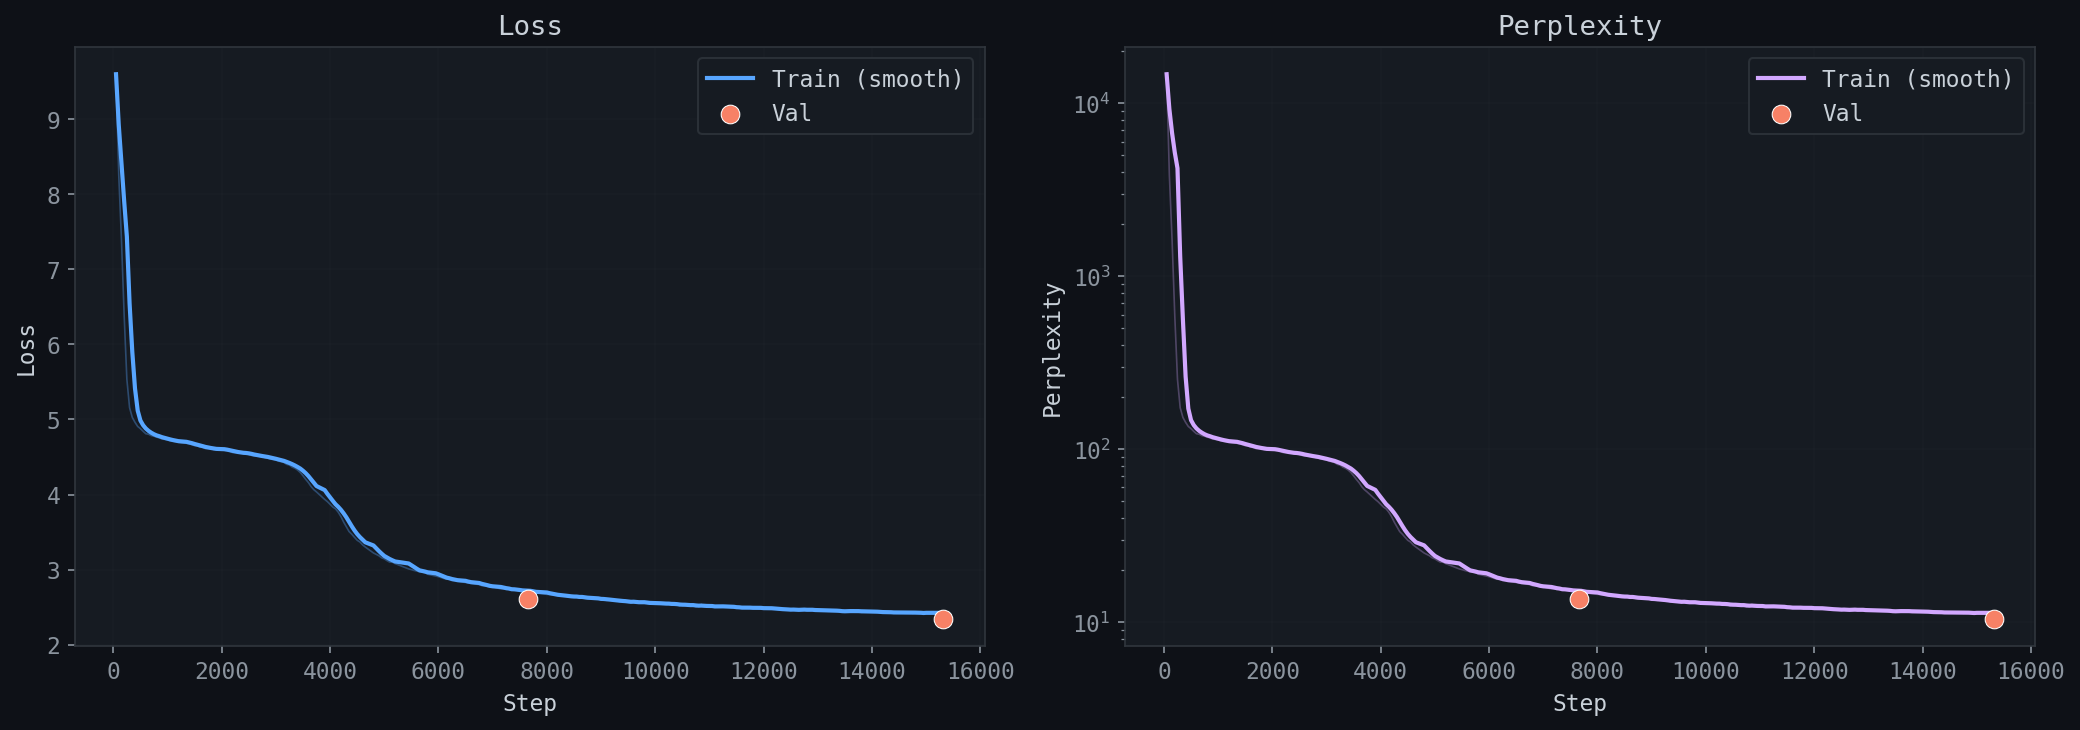
\includegraphics[width=\linewidth]{../metrics/loss_perplexity.png}
		\caption{Training and Validation Loss/Perplexity.}
		\label{fig:loss_perp}
	\end{figure}
	
	\begin{figure}[!htb]
		\centering
		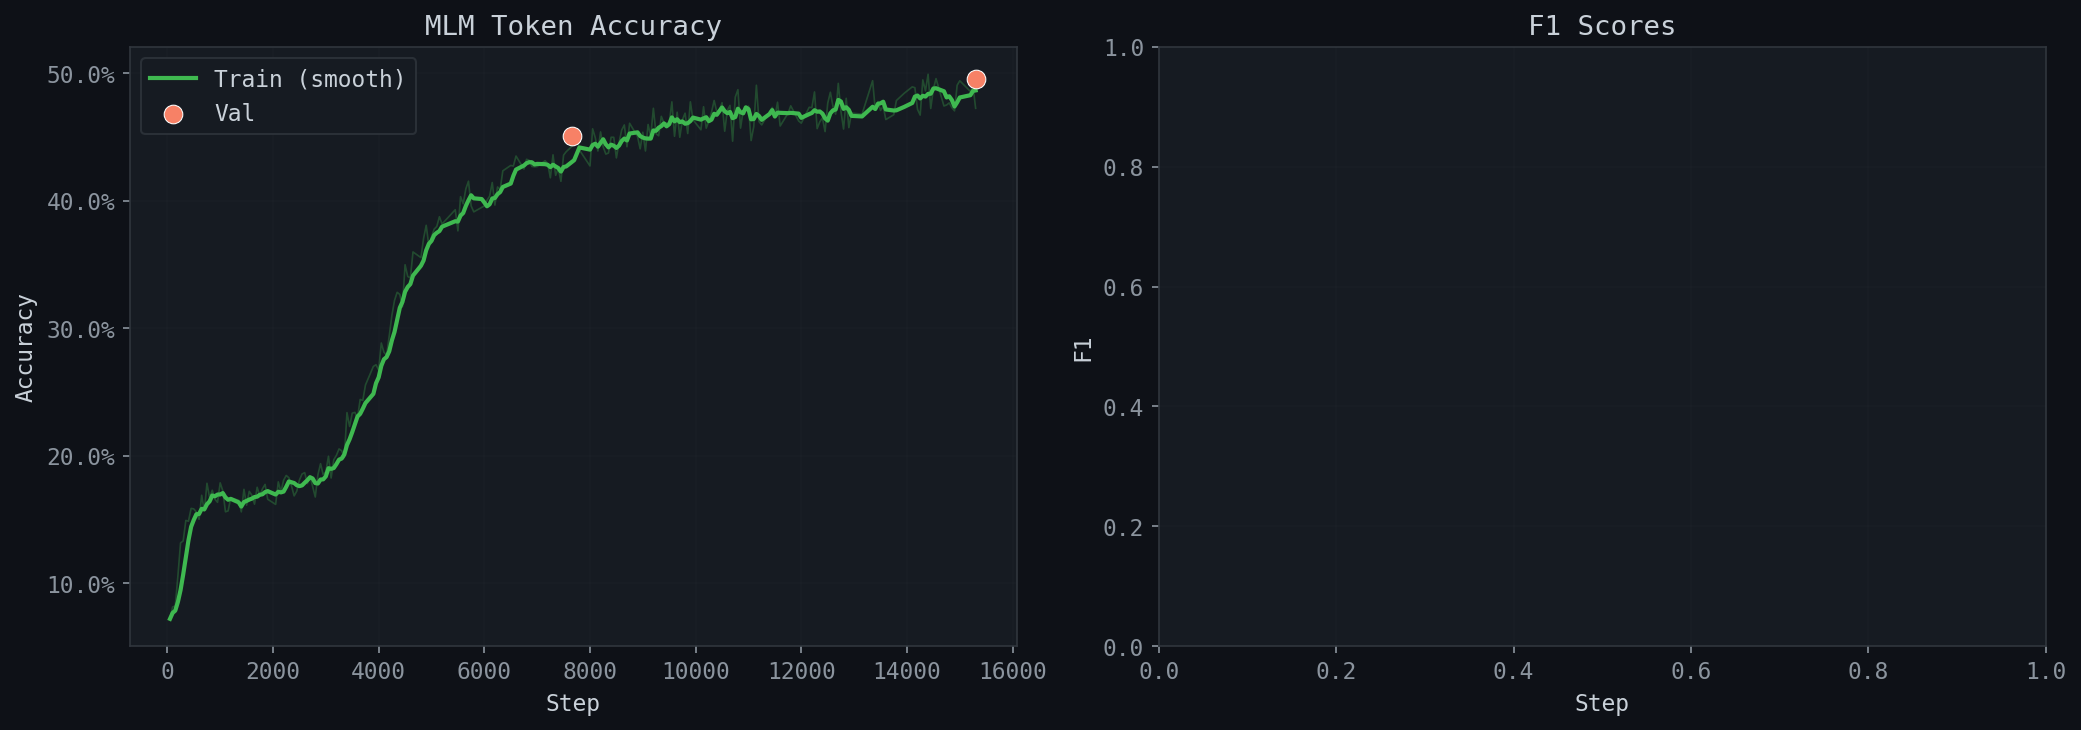
\includegraphics[width=\linewidth]{../metrics/accuracy_f1.png}
		\caption{MLM Accuracy and F1 Score evolution.}
		\label{fig:acc_f1}
	\end{figure}
	
	\begin{figure}[!htb]
		\centering
		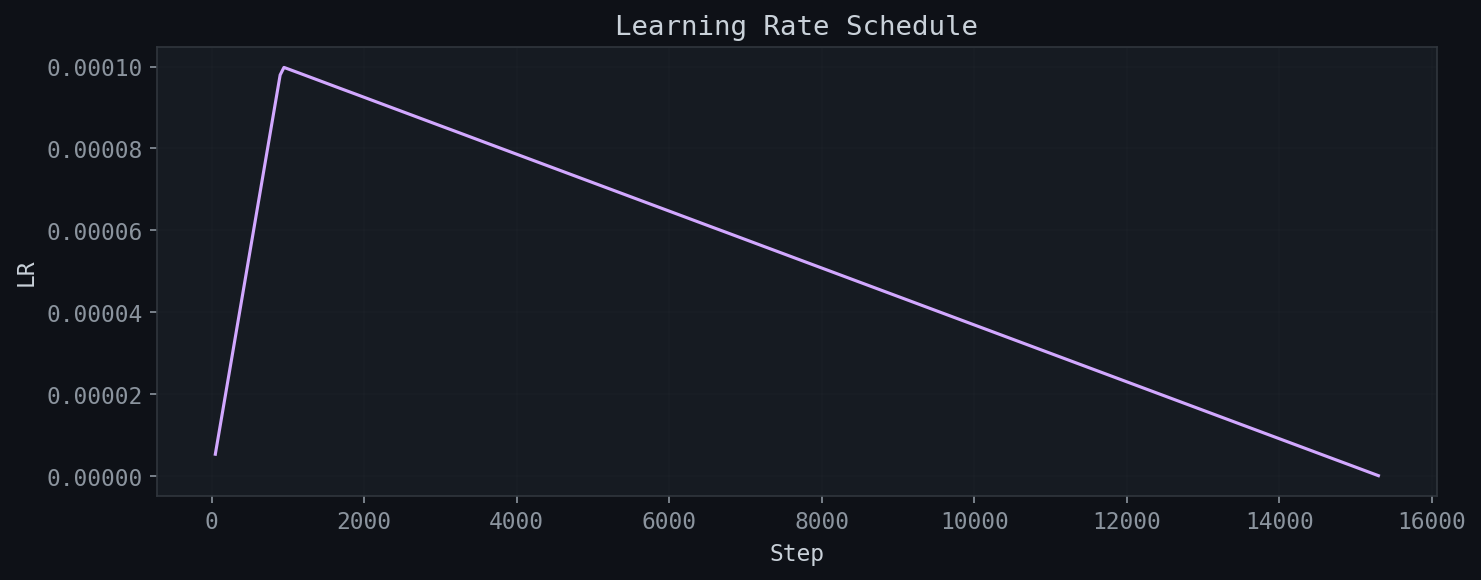
\includegraphics[width=\linewidth]{../metrics/learning_rate.png}
		\caption{Learning rate schedule (linear decay with warmup).}
		\label{fig:lr}
	\end{figure}
	
	The learning rate schedule (Figure~\ref{fig:lr}) uses a linear warmup over the first 6\%
	of steps, then decays linearly to zero.
	
	\begin{figure}[!htb]
		\centering
		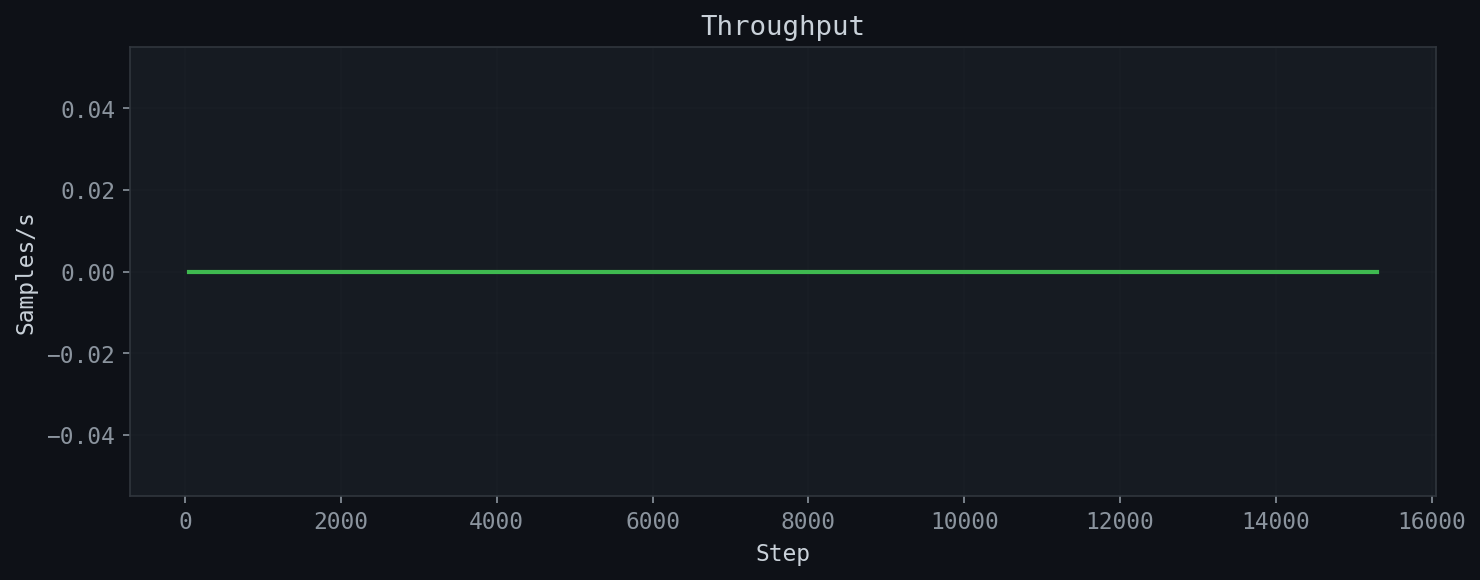
\includegraphics[width=\linewidth]{../metrics/throughput.png}
		\caption{Training throughput (samples/sec).}
		\label{fig:throughput}
	\end{figure}
	
	\subsection{Architecture Diagnostics}
	
	\begin{figure}[!htb]
		\centering
		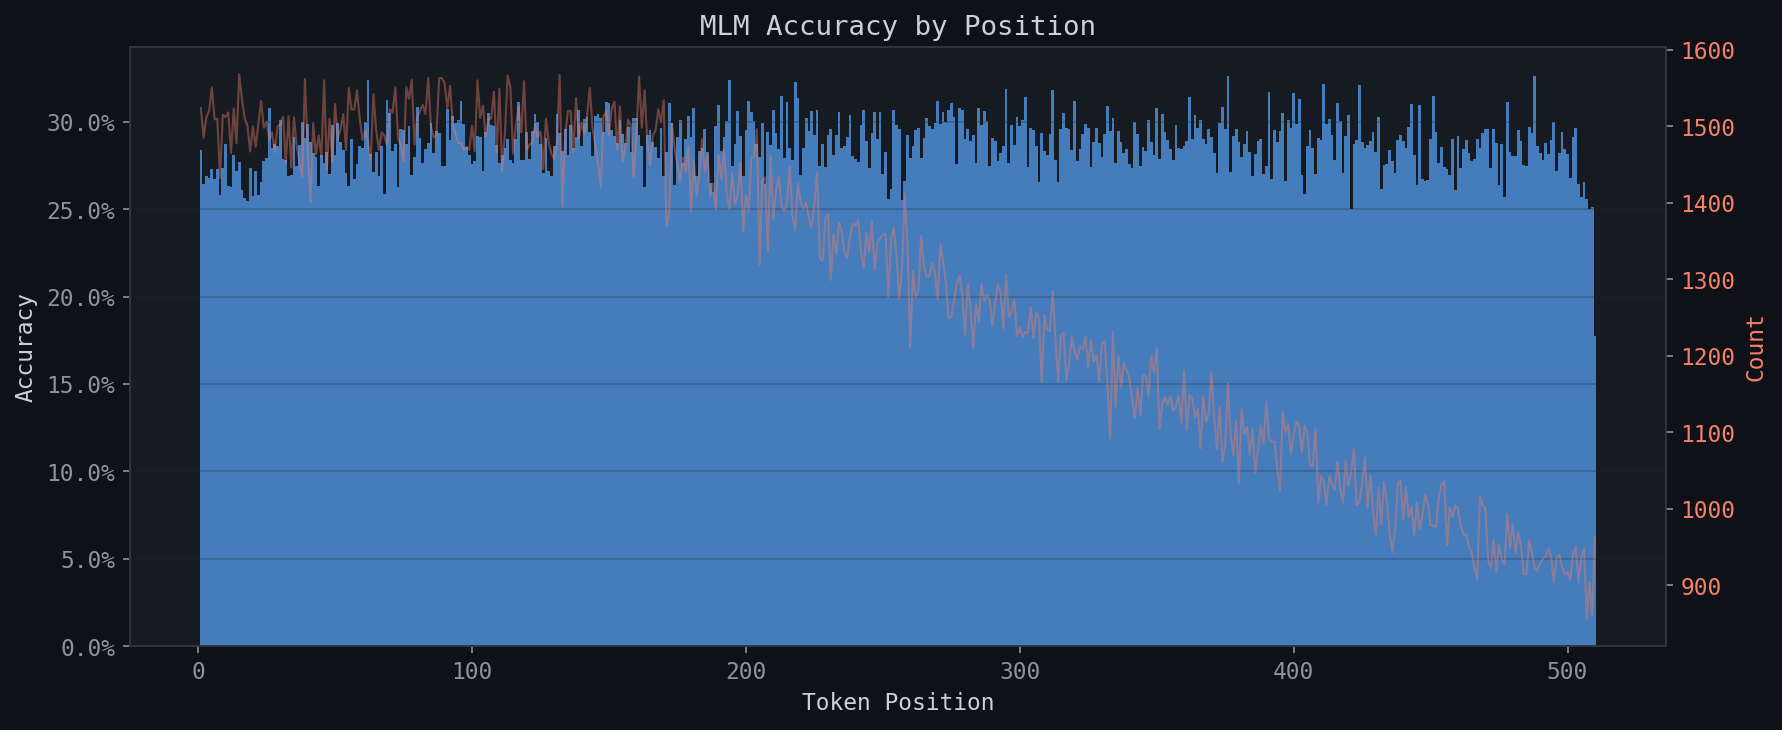
\includegraphics[width=\linewidth]{../metrics/accuracy_by_position.png}
		\caption{MLM Accuracy by token position in sequence.}
		\label{fig:pos_acc}
	\end{figure}
	
	\begin{figure}[!htb]
		\centering
		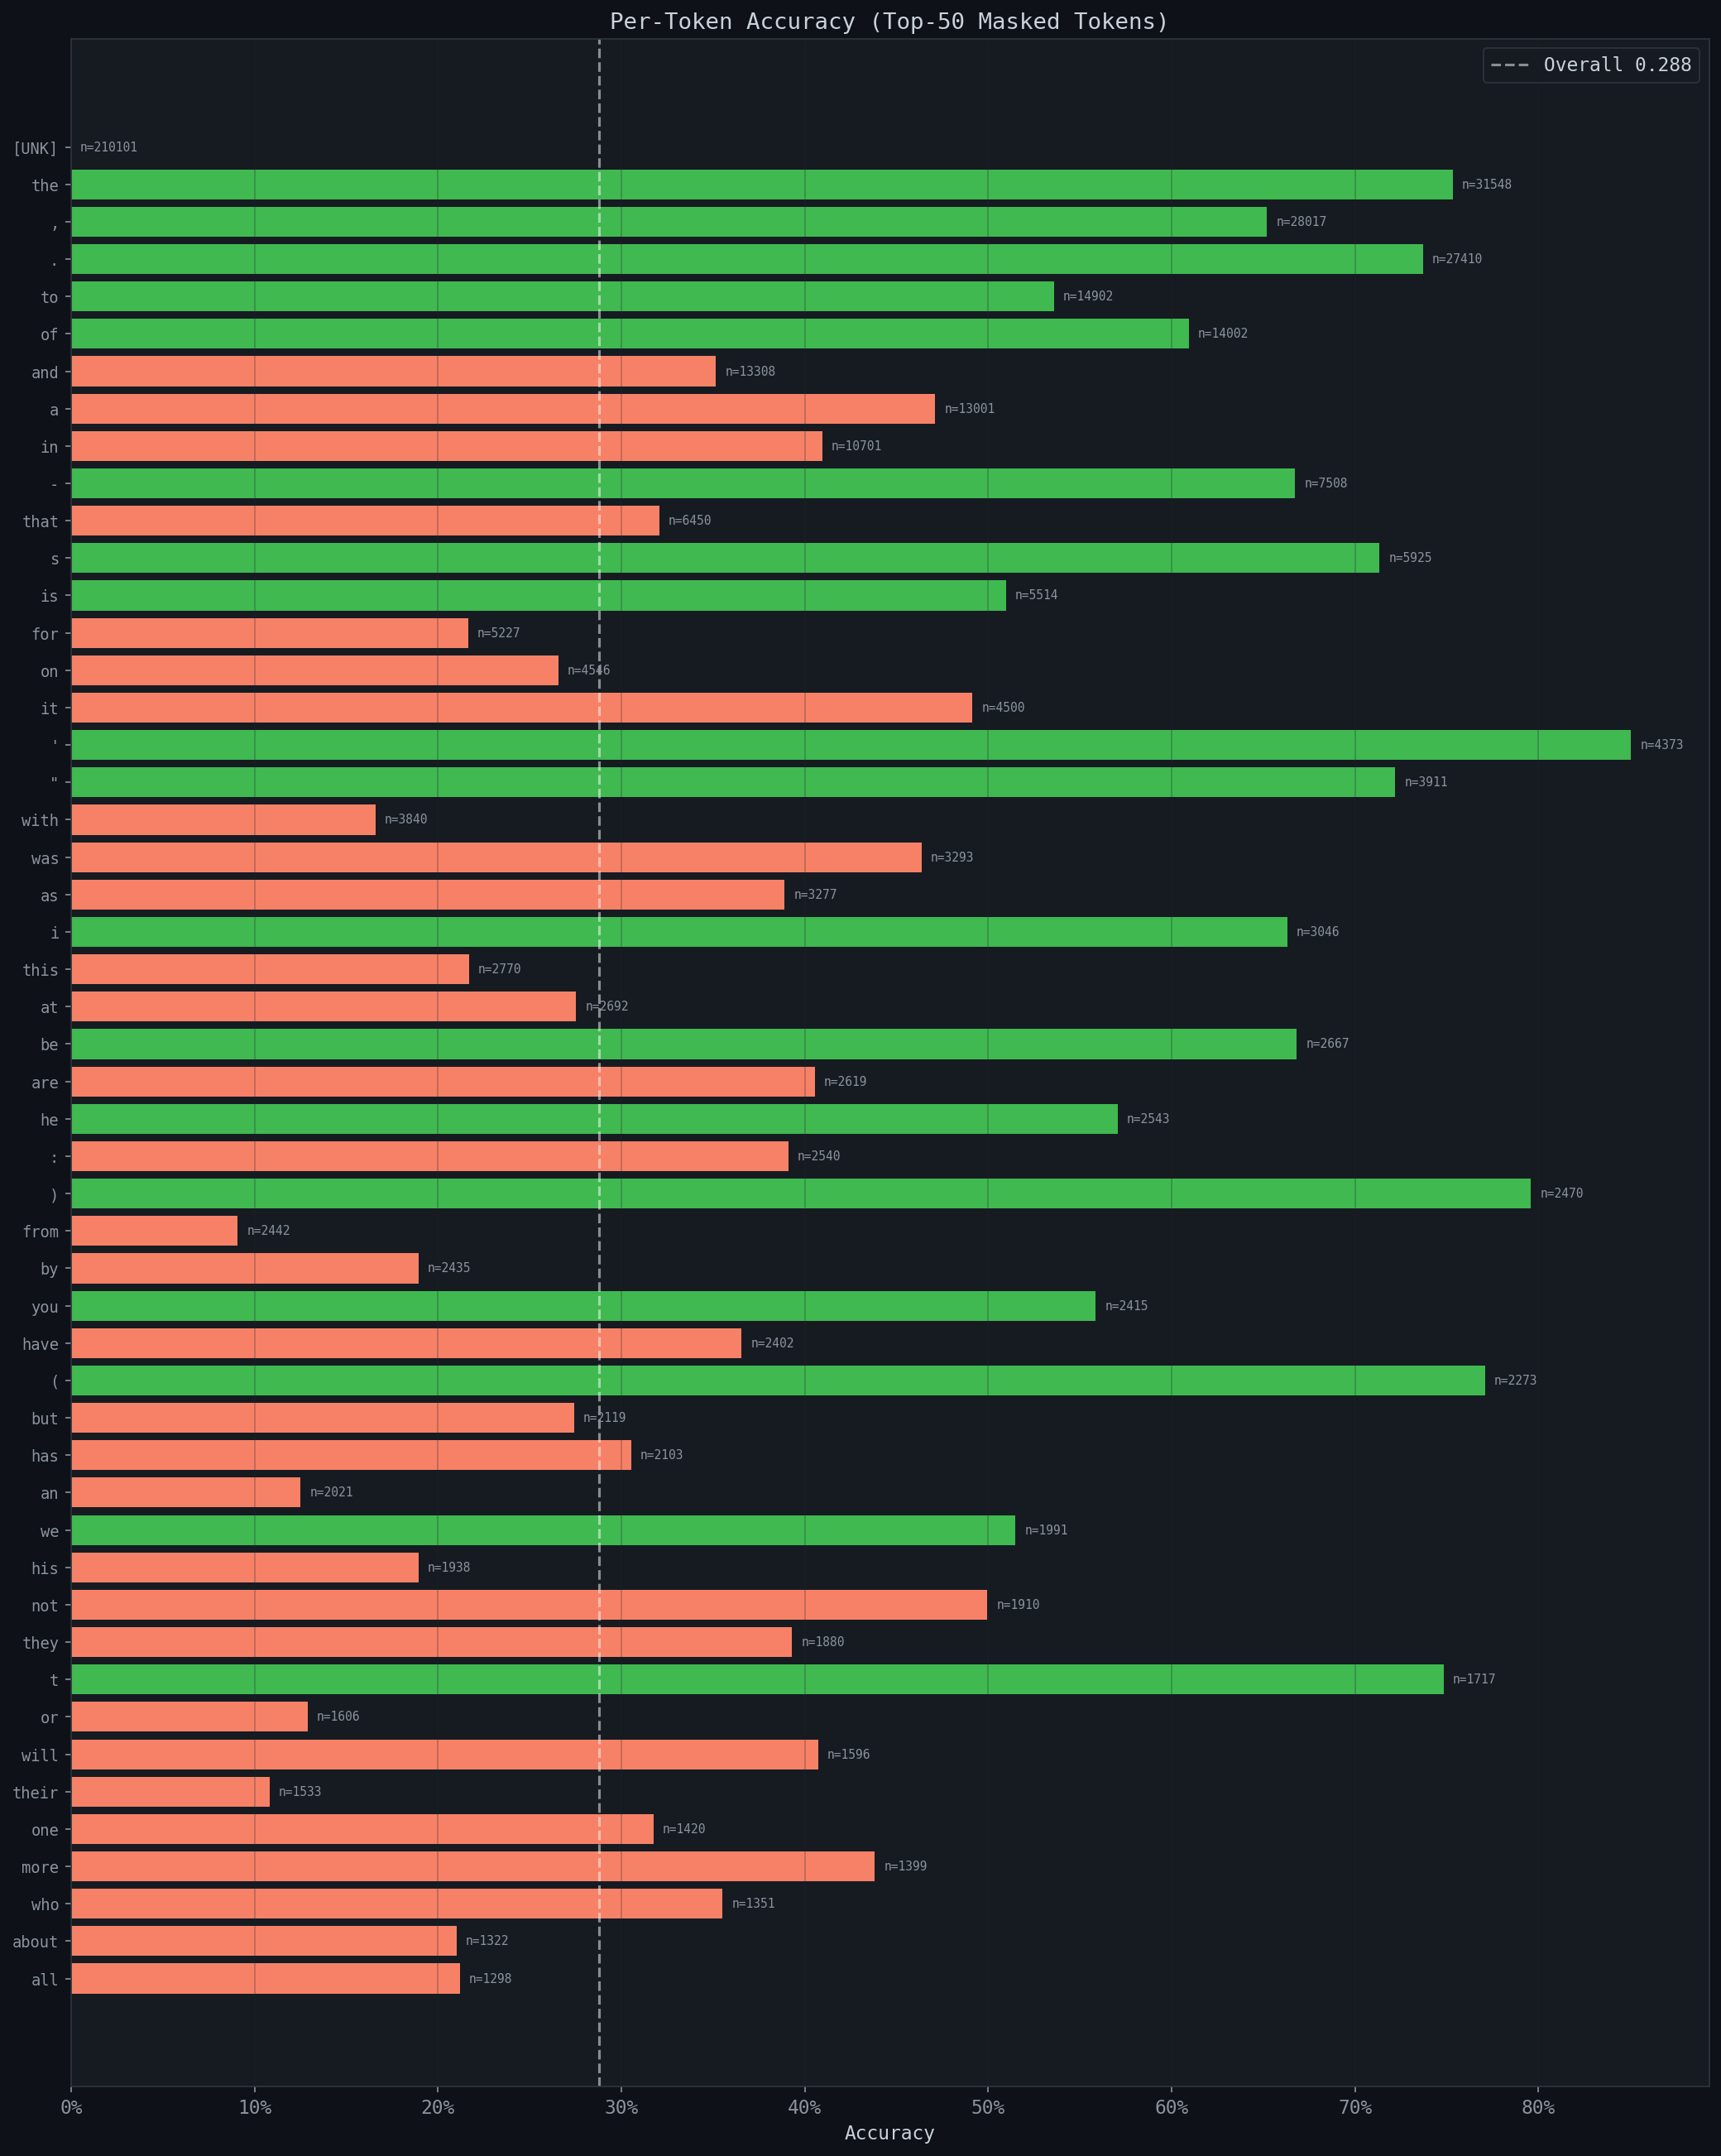
\includegraphics[width=\linewidth]{../metrics/per_token_accuracy.png}
		\caption{Accuracy for top-K frequent tokens.}
		\label{fig:per_tok}
	\end{figure}
	
	\begin{figure}[!htb]
		\centering
		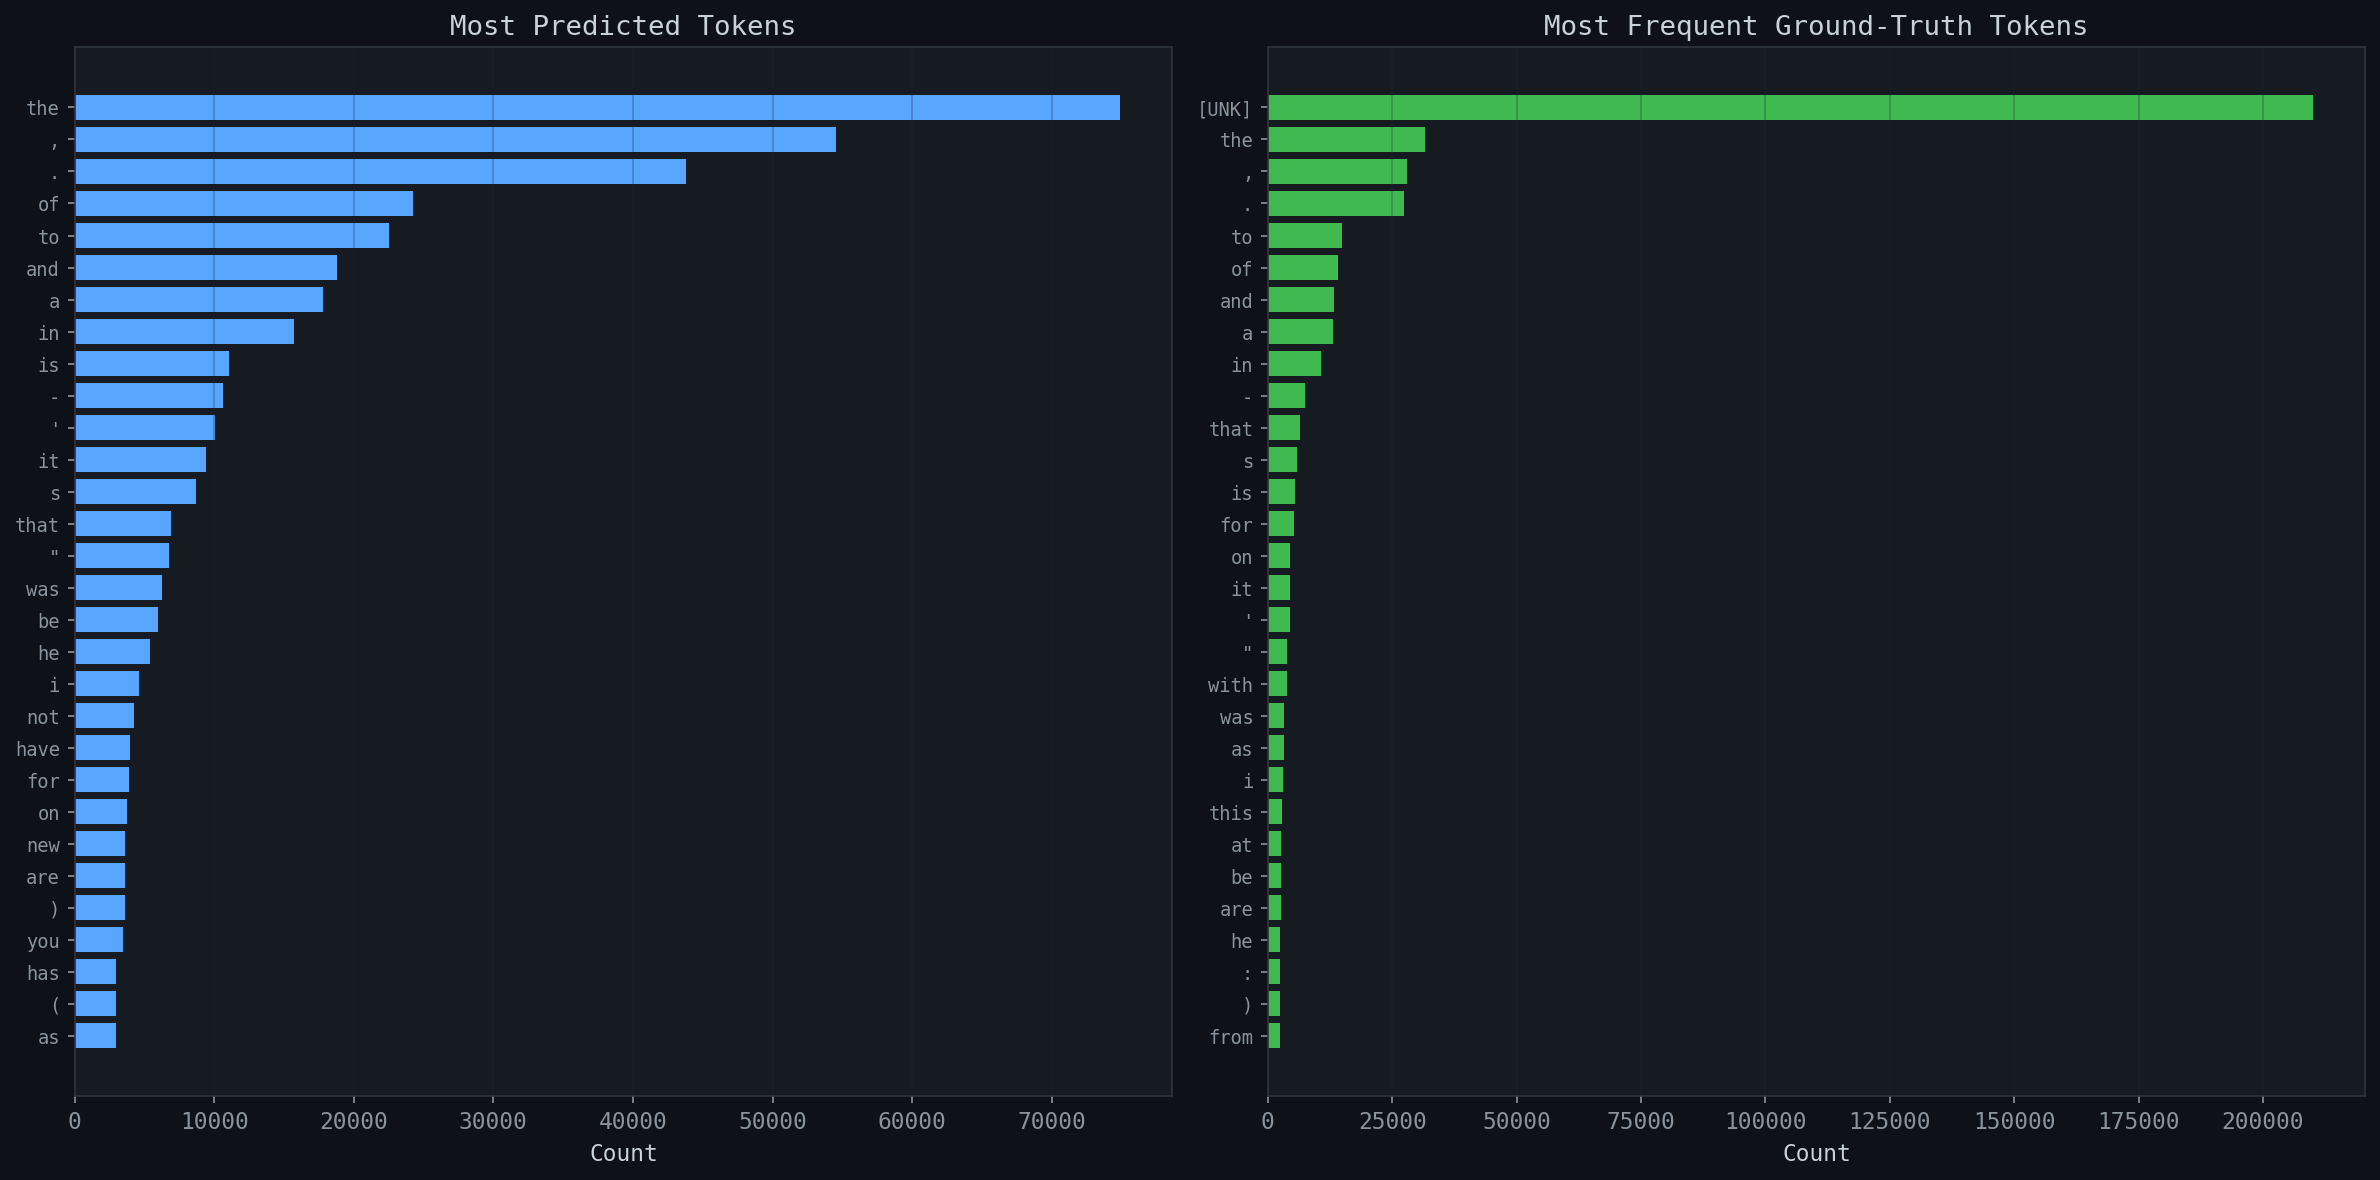
\includegraphics[width=\linewidth]{../metrics/token_distribution.png}
		\caption{Distribution of predicted vs.\ gold tokens.}
		\label{fig:tok_dist}
	\end{figure}
	
	\begin{figure}[!htb]
		\centering
		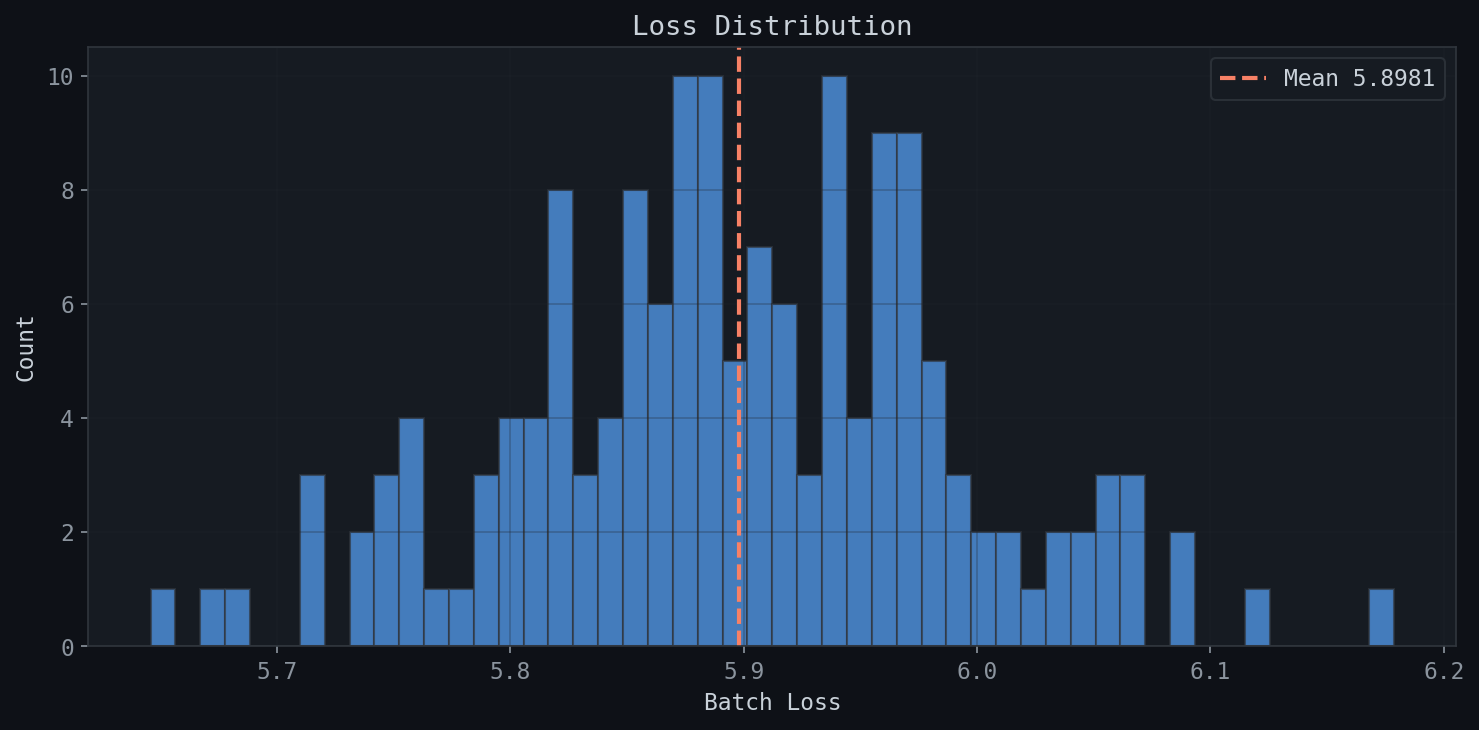
\includegraphics[width=\linewidth]{../metrics/loss_distribution.png}
		\caption{Cross-entropy loss distribution across samples.}
		\label{fig:loss_dist}
	\end{figure}
	
	The loss distribution (Figure~\ref{fig:loss_dist}) shows a symmetric spread around a
	mean batch loss of 5.90.
	
	\begin{figure}[!htb]
		\centering
		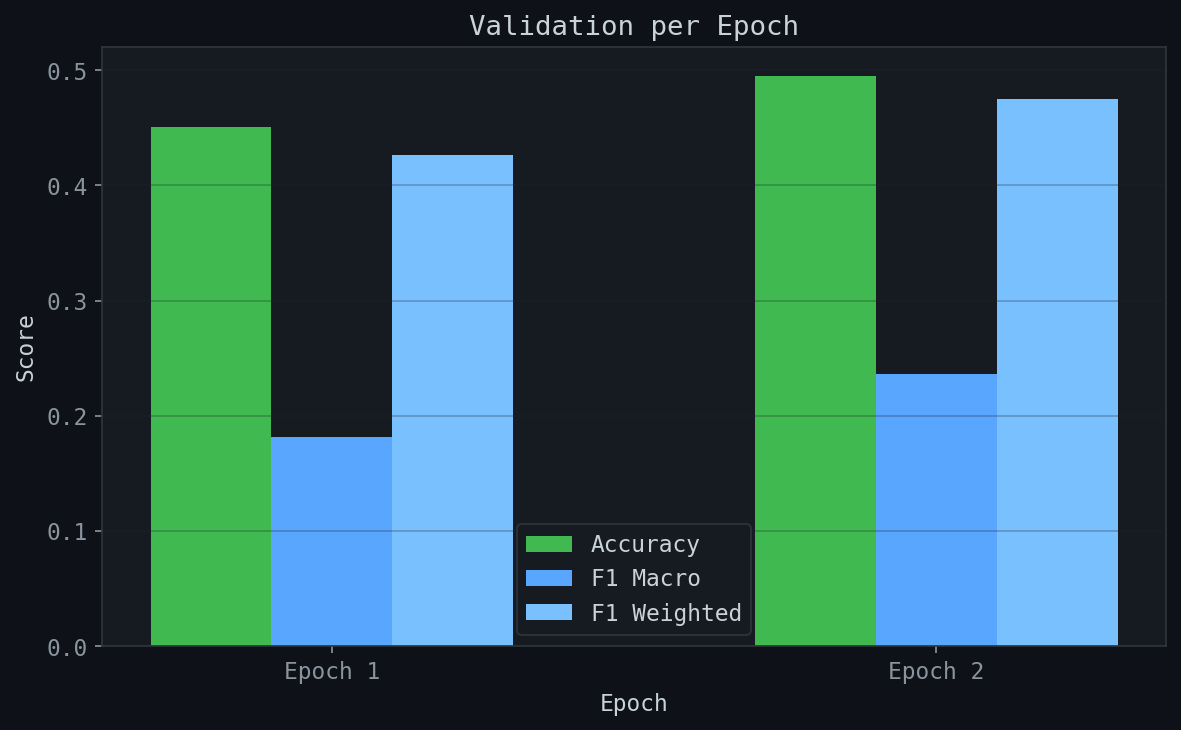
\includegraphics[width=\linewidth]{../metrics/epoch_summary.png}
		\caption{Validation metrics per epoch.}
		\label{fig:epoch}
	\end{figure}
	
	% ======================================================================
	\section{Phase 2: Dataset Bias Profiling}
	% ======================================================================
	We analyzed the Bias-in-Bios dataset (396k biographies) to identify inherent gender skews
	across 28 professions. The overall split shows a slight male majority (53.9\% vs.\ 46.1\%),
	but per-profession distributions reveal far more extreme imbalances.
	
	\begin{figure}[!htb]
		\centering
		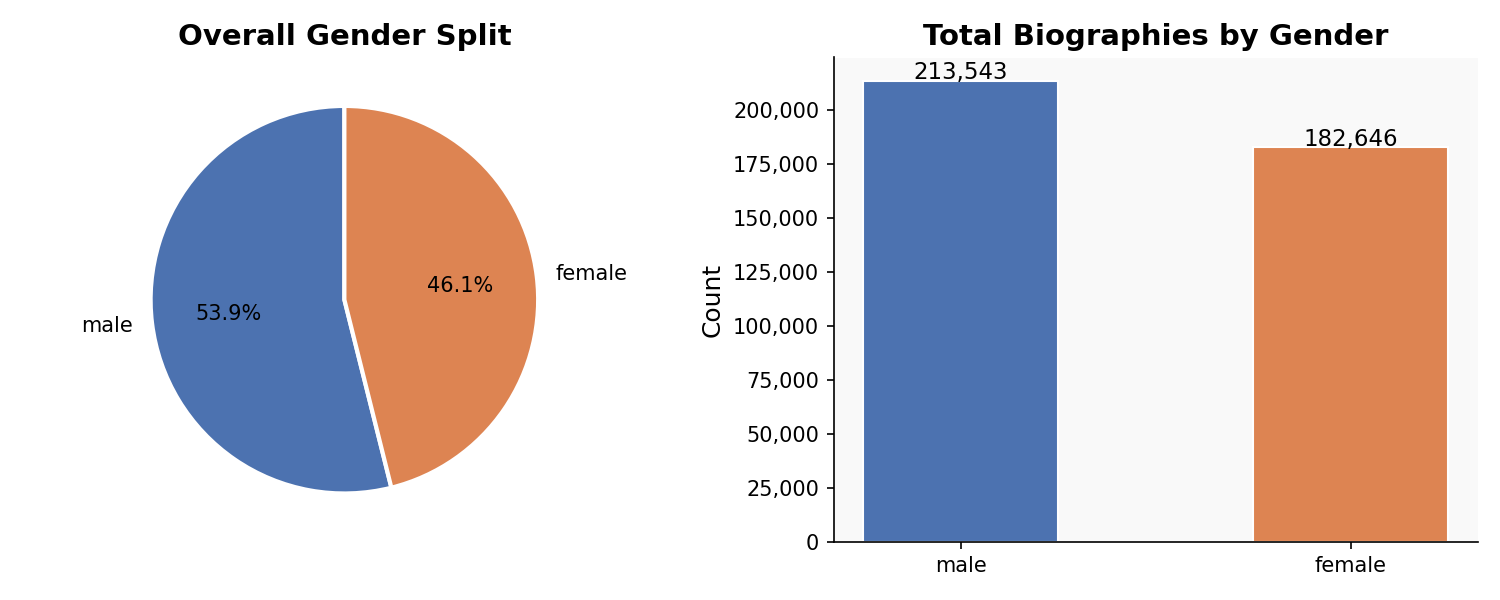
\includegraphics[width=\linewidth]{../biasbios_metrics/08_overall_balance.png}
		\caption{Overall dataset gender balance.}
		\label{fig:balance}
	\end{figure}
	
	\begin{figure}[!htb]
		\centering
		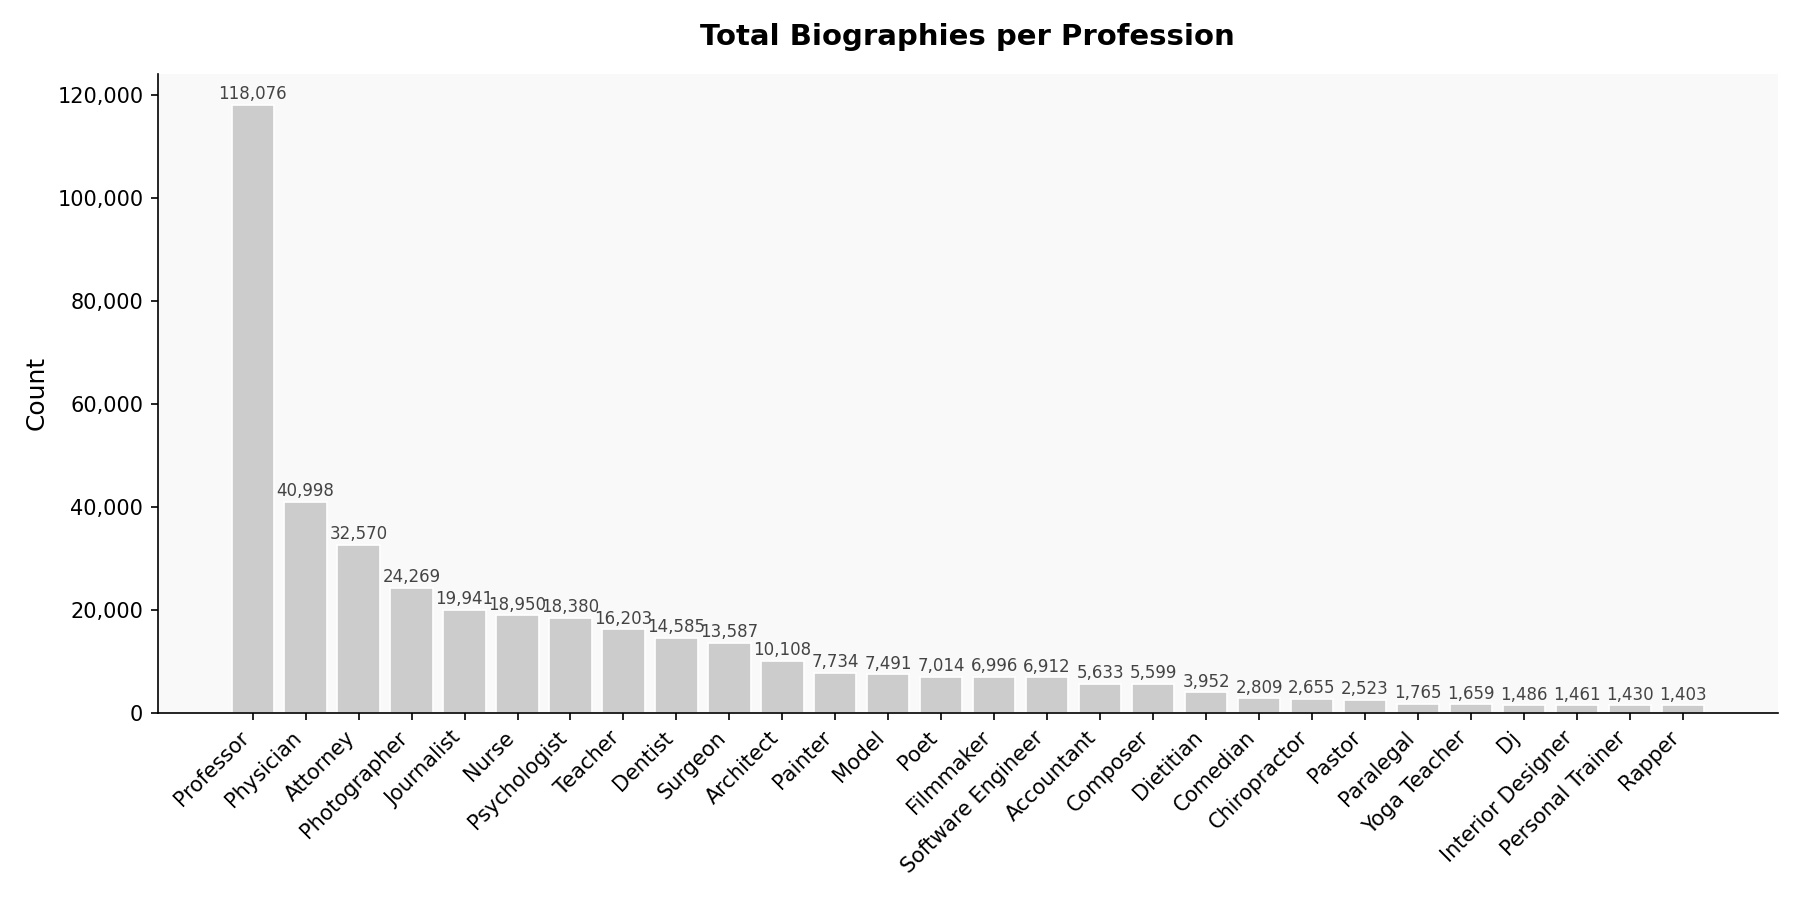
\includegraphics[width=\linewidth]{../biasbios_metrics/01_profession_counts.png}
		\caption{Total biographies per profession (class imbalance).}
		\label{fig:prof_counts}
	\end{figure}
	
	\begin{figure}[!htb]
		\centering
		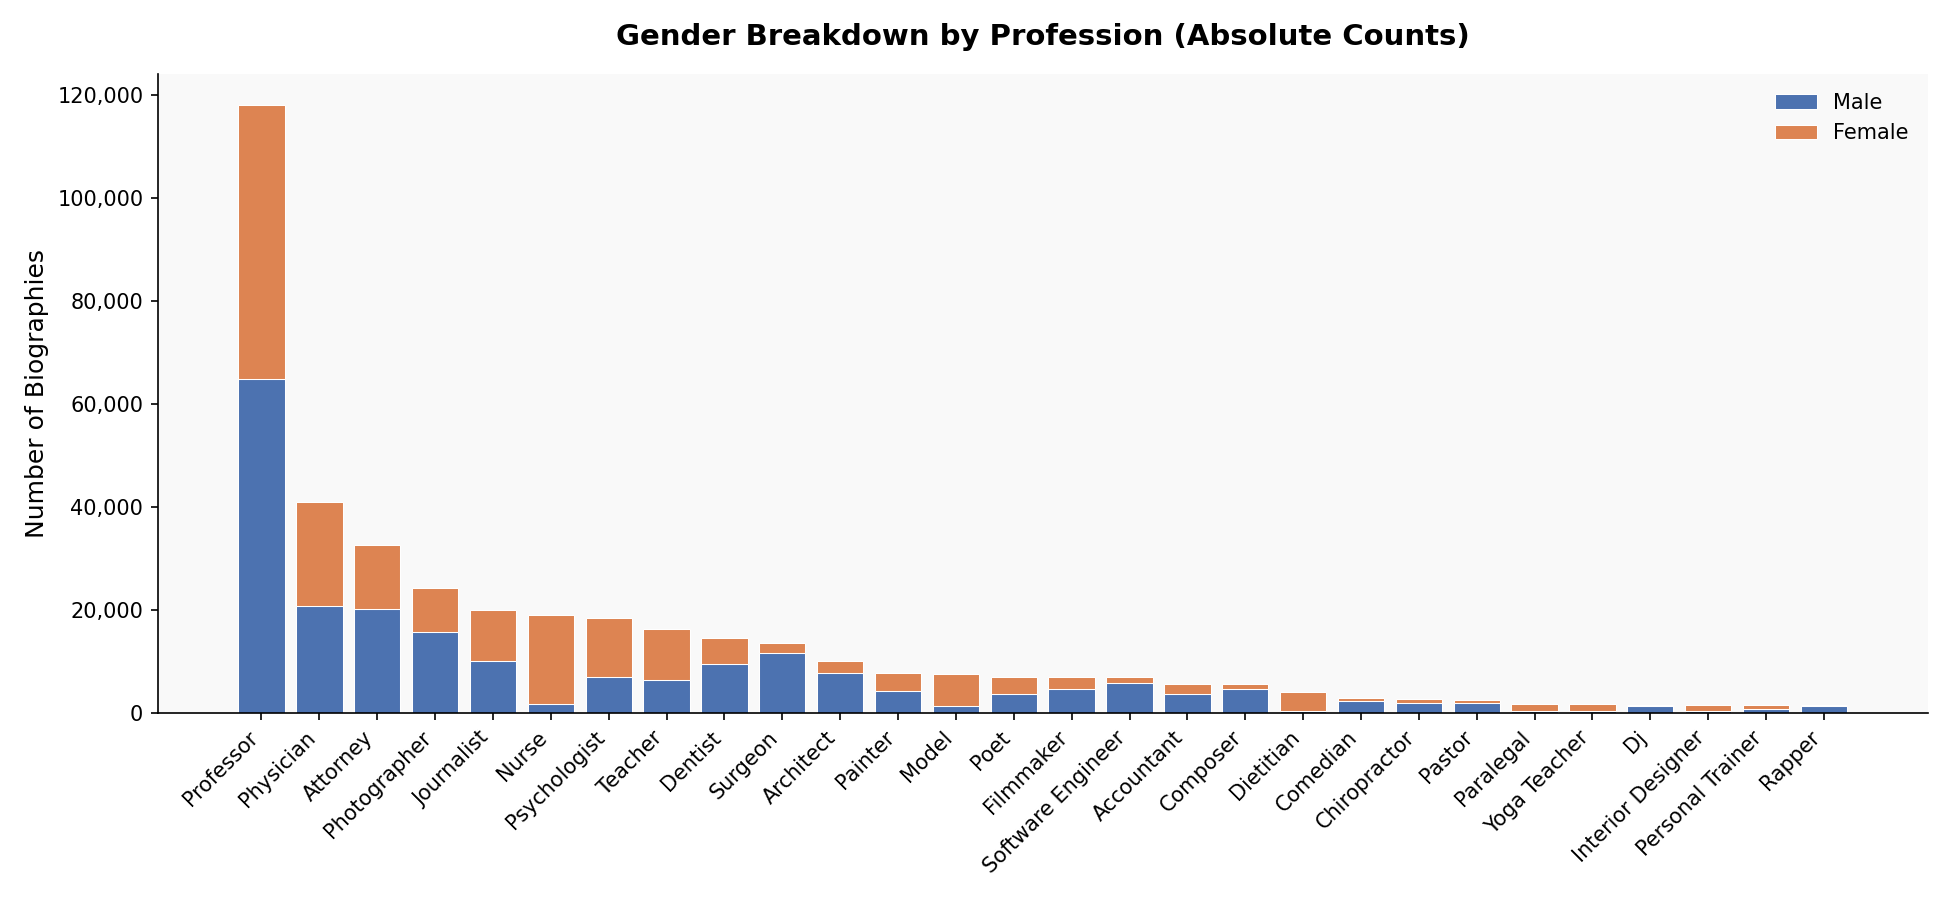
\includegraphics[width=\linewidth]{../biasbios_metrics/02_gender_breakdown_stacked.png}
		\caption{Absolute gender counts per profession.}
		\label{fig:gender_stacked}
	\end{figure}
	
	\begin{figure}[!htb]
		\centering
		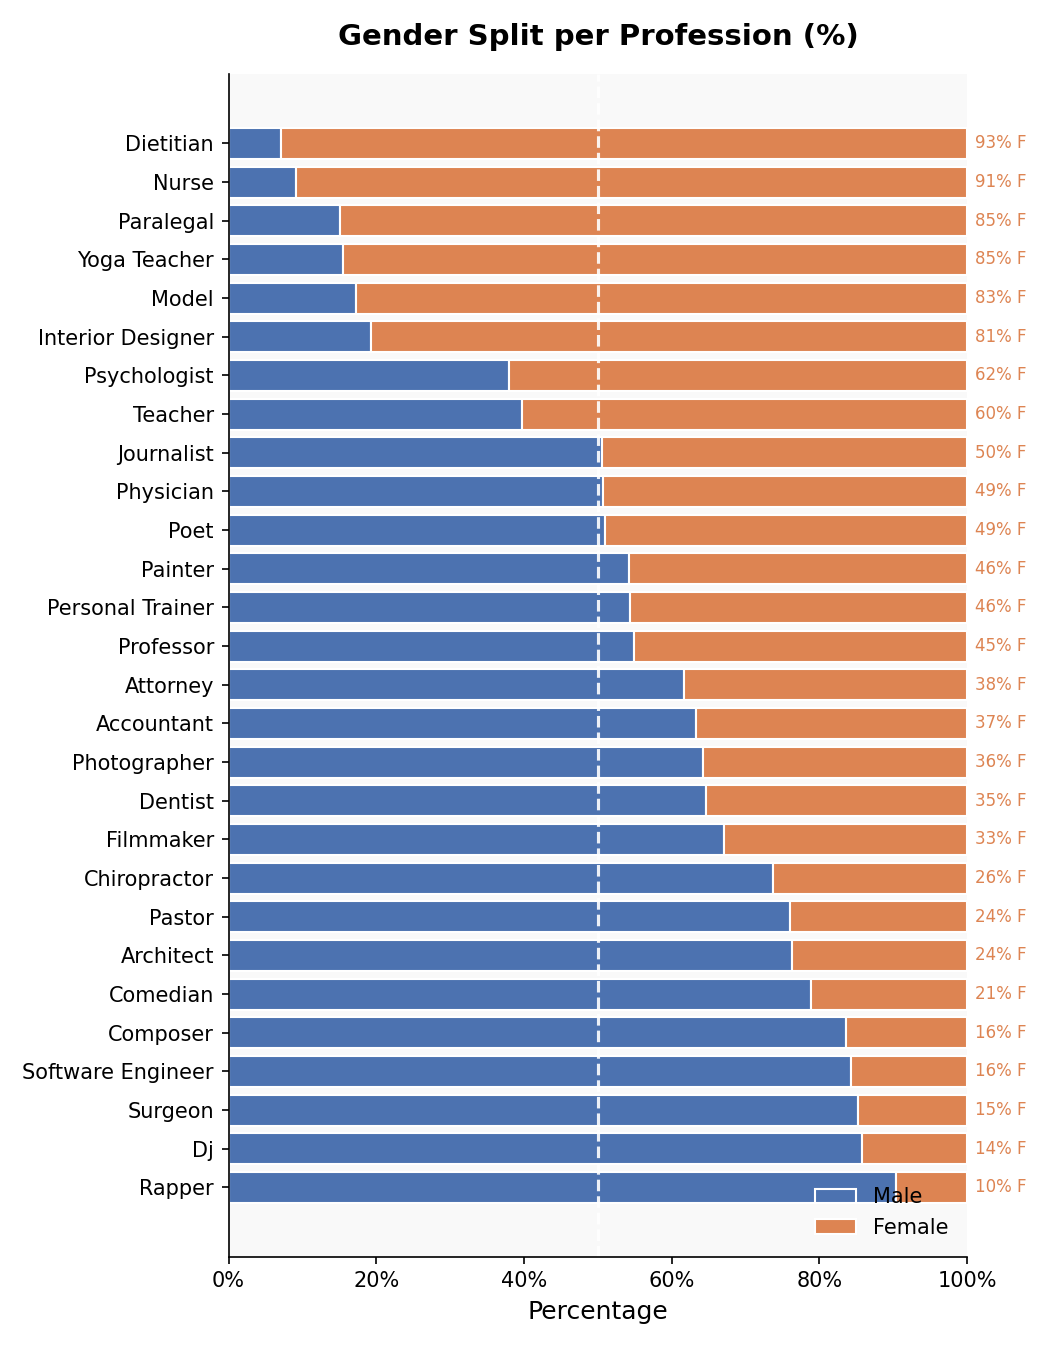
\includegraphics[width=\linewidth]{../biasbios_metrics/03_gender_pct_horizontal.png}
		\caption{Percentage split of genders per profession.}
		\label{fig:gender_pct}
	\end{figure}
	
	\begin{figure}[!htb]
		\centering
		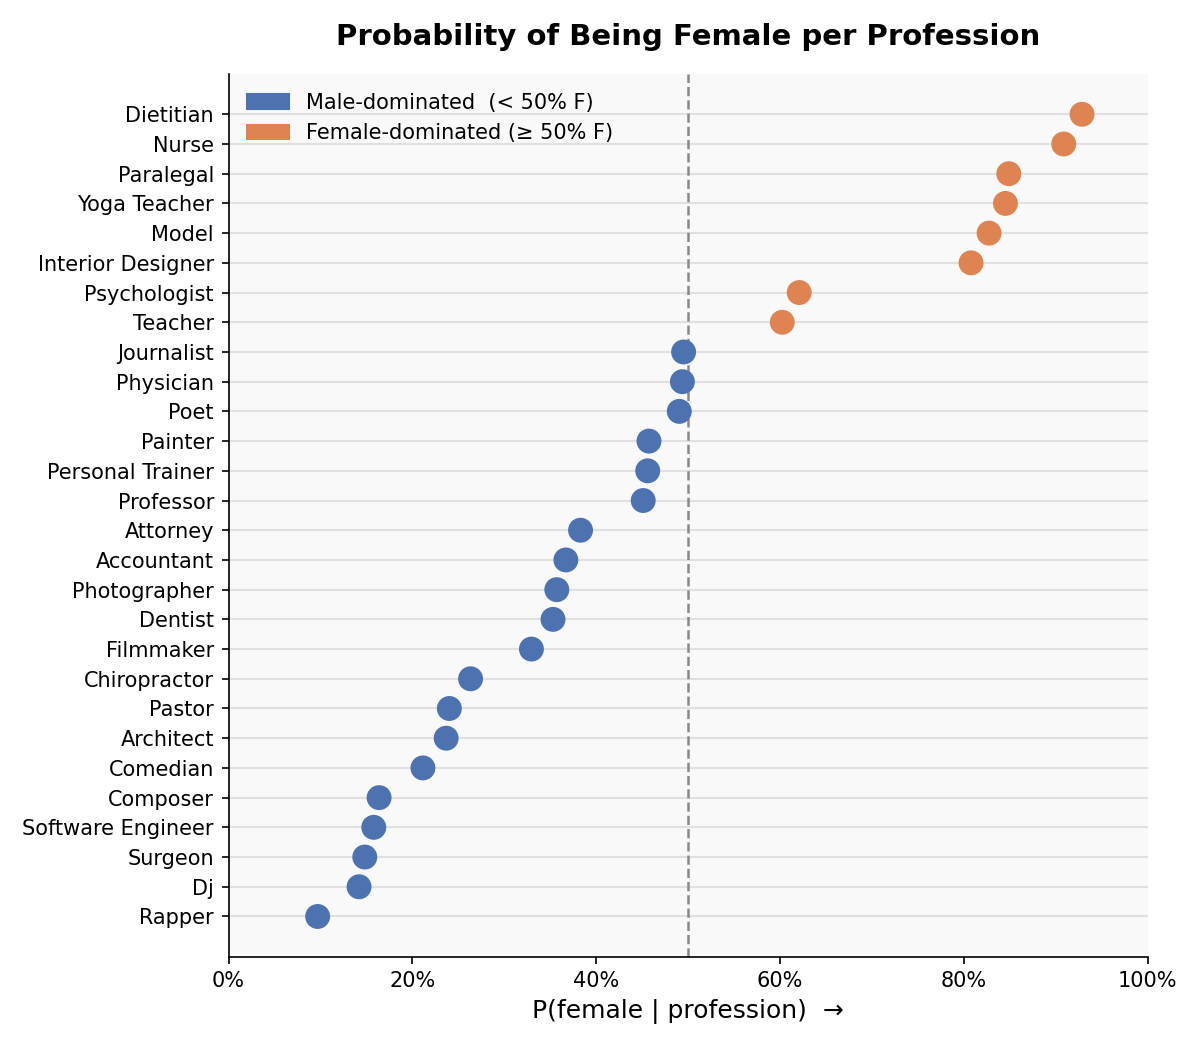
\includegraphics[width=\linewidth]{../biasbios_metrics/04_prob_female_dotplot.png}
		\caption{Probability of a biography being female given the profession.}
		\label{fig:prob_female}
	\end{figure}
	
	\begin{figure}[!htb]
		\centering
		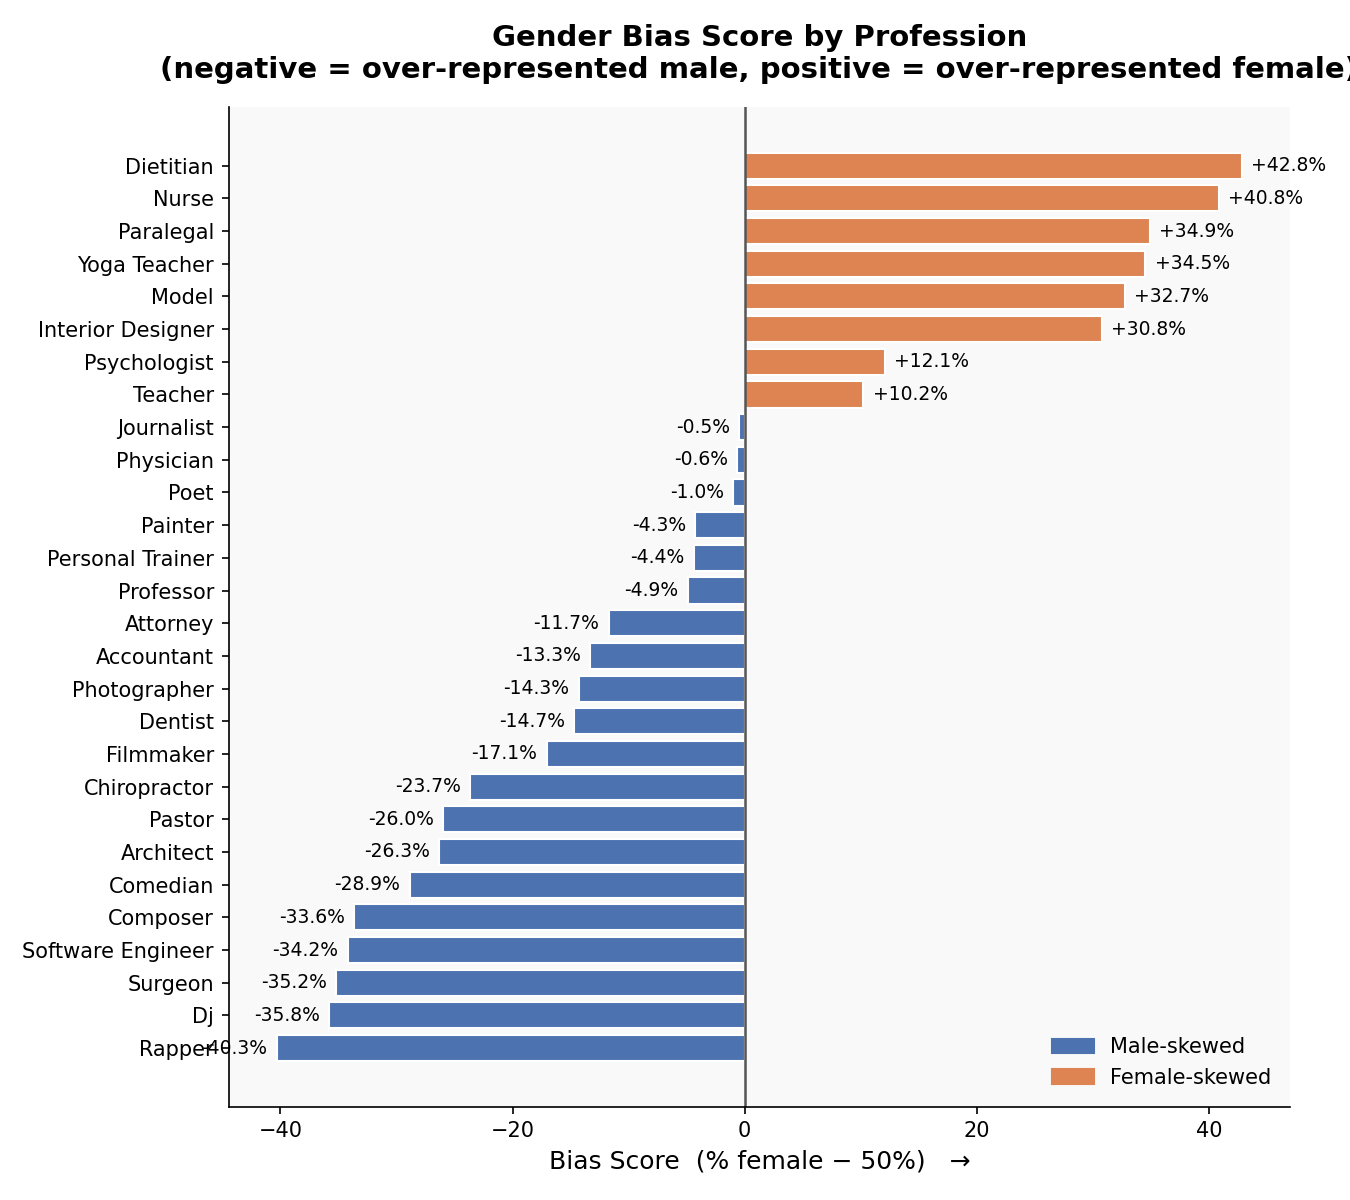
\includegraphics[width=\linewidth]{../biasbios_metrics/05_bias_diverging.png}
		\caption{Diverging Bias Score (\%Female $-$ 50\%).}
		\label{fig:bias_div}
	\end{figure}
	
	\begin{figure}[!htb]
		\centering
		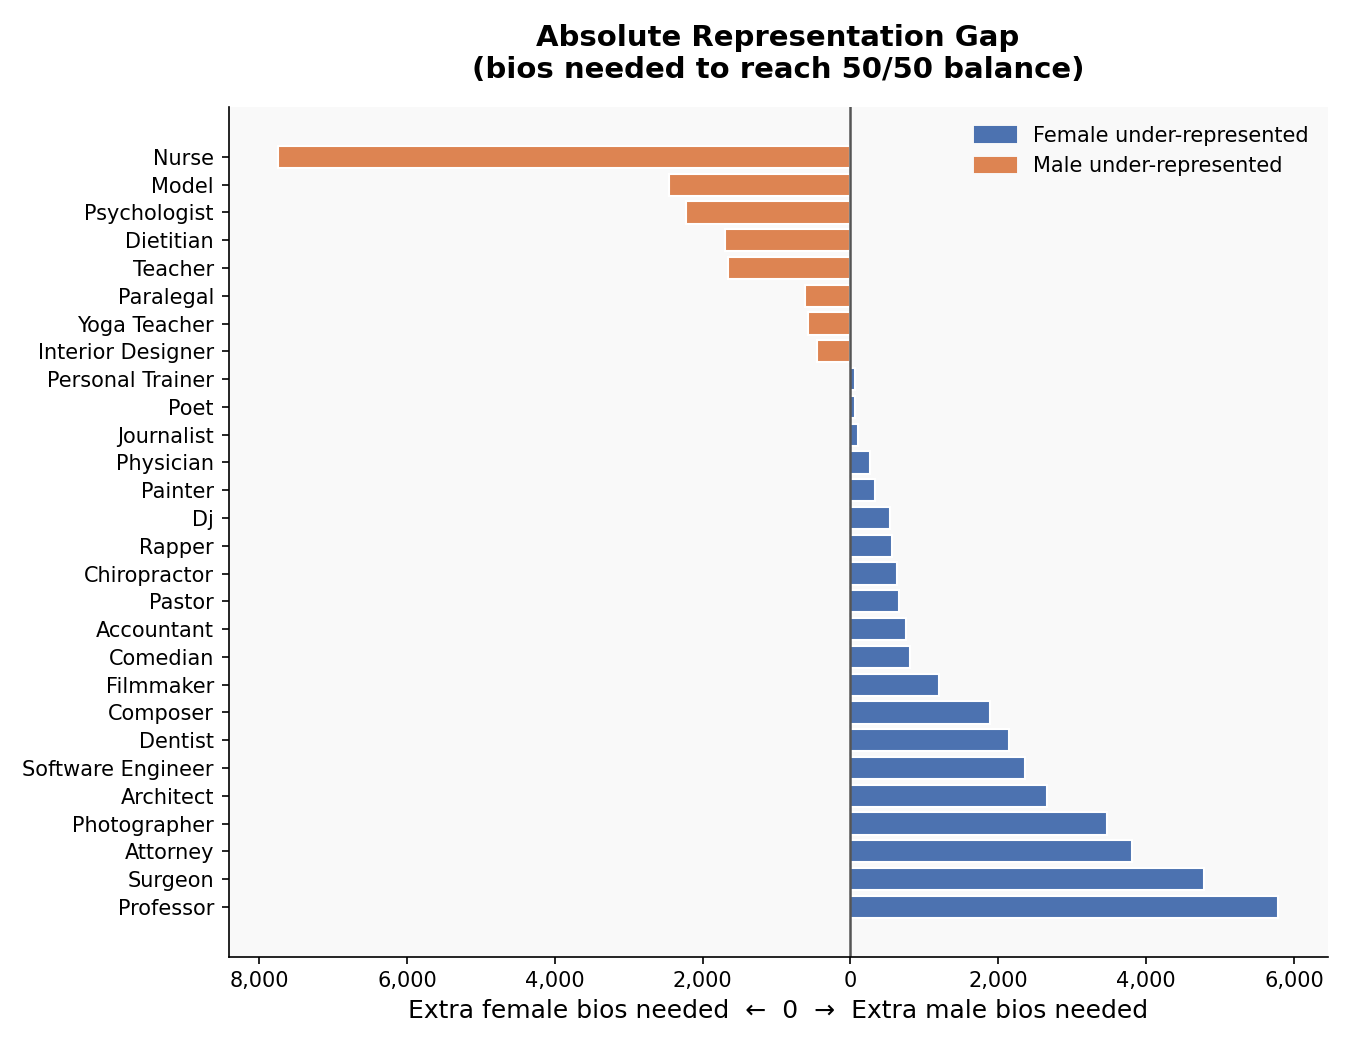
\includegraphics[width=\linewidth]{../biasbios_metrics/06_absolute_gap.png}
		\caption{Absolute representation gap (samples needed for parity).}
		\label{fig:abs_gap}
	\end{figure}
	
	\begin{figure}[!htb]
		\centering
		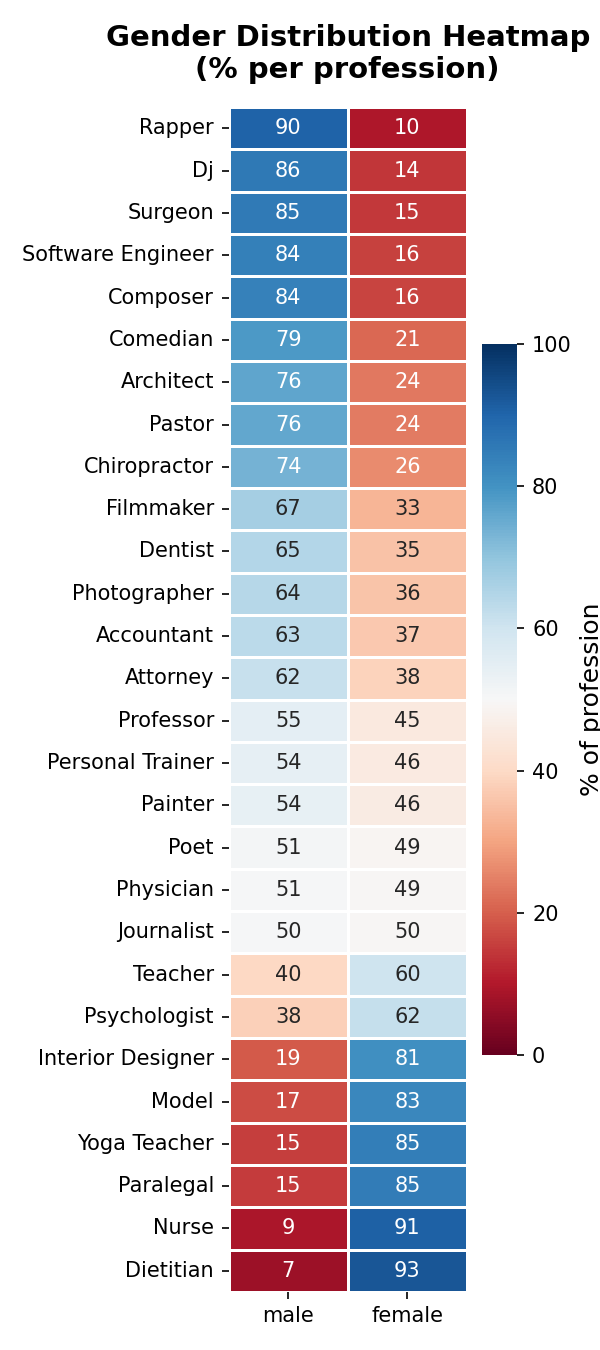
\includegraphics[width=\linewidth]{../biasbios_metrics/07_gender_heatmap.png}
		\caption{Gender distribution heatmap (\% per profession).}
		\label{fig:heatmap}
	\end{figure}
	
	The heatmap (Figure~\ref{fig:heatmap}) shows \textit{Rapper} (90\% male) and
	\textit{Dietitian} (93\% female) at the extremes, with \textit{Journalist} and
	\textit{Physician} near parity.
	
	% ======================================================================
	\section{Phase 3 \& 4: Biased vs.\ Debiased Models}
	% ======================================================================
	The ``Biased'' model was trained with stereotypical oversampling; the ``Debiased'' model
	used counterfactual augmentation and balancing.
	
	\subsection{Fine-tuning Architecture and Process}
	
	\paragraph{Classification head.}
	The \texttt{[CLS]} token's 768-dim hidden state passes through dropout ($p=0.1$) and a
	linear projection to 28 logits. During inference, softmax and argmax select the predicted
	profession.
	
	\begin{figure}[!htb]
		\centering
		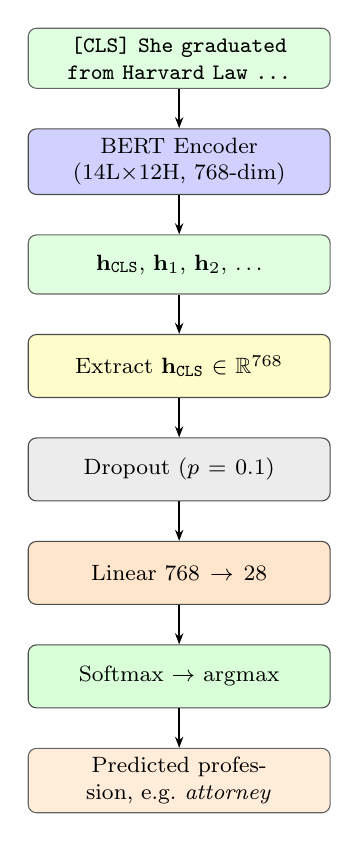
\begin{tikzpicture}[node distance=0.5cm, every node/.style={font=\scriptsize}]
			\node[cdatablock](input){\texttt{[CLS] She graduated from Harvard Law \ldots}};
			\node[cwideblock,below=of input,fill=blue!18](encoder){BERT Encoder (14L$\times$12H, 768-dim)};
			\node[cdatablock,below=of encoder](hidden){$\mathbf{h}_{\texttt{CLS}},\,\mathbf{h}_1,\,\mathbf{h}_2,\,\ldots$};
			\node[cblock,below=of hidden,fill=yellow!20](cls){Extract $\mathbf{h}_{\texttt{CLS}}\!\in\!\mathbb{R}^{768}$};
			\node[cblock,below=of cls,fill=gray!15](drop){Dropout ($p\!=\!0.1$)};
			\node[cblock,below=of drop,fill=orange!20](linear){Linear $768\!\to\!28$};
			\node[cblock,below=of linear,fill=green!15](softmax){Softmax $\to$ argmax};
			\node[coutblock,below=of softmax](output){Predicted profession, e.g.\ \textit{attorney}};
			\draw[arrow](input)--(encoder);\draw[arrow](encoder)--(hidden);
			\draw[arrow](hidden)--(cls);\draw[arrow](cls)--(drop);
			\draw[arrow](drop)--(linear);\draw[arrow](linear)--(softmax);
			\draw[arrow](softmax)--(output);
		\end{tikzpicture}
		\caption{Fine-tuning architecture. Only \texttt{[CLS]} is forwarded to the head.}
		\label{fig:finetune_arch}
	\end{figure}
	
	\paragraph{Training settings.}
	Both models share: AdamW, lr $2\times10^{-5}$, linear warm-up (6\%), weight decay $0.01$,
	\texttt{fp16}, gradient clip 1.0, 3 epochs. The only difference is the training set.
	
	\subsection{Debiasing: Counterfactual Data Augmentation}
	\label{sec:debiasing}
	
	\subsubsection*{Step 1 — Gender Balancing}
	For each profession, male and female subsets are sub-sampled to their common minimum,
	producing a perfectly balanced dataset.
	
	\subsubsection*{Step 2 — CDA}
	Each biography is duplicated with gendered cues swapped
	(\textit{he}$\leftrightarrow$\textit{she}, \textit{Mr.}$\leftrightarrow$\textit{Ms.},
	etc.). The profession label is preserved; the gender label is flipped.
	
	\begin{figure}[!htb]
		\centering
		\resizebox{\linewidth}{!}{%
			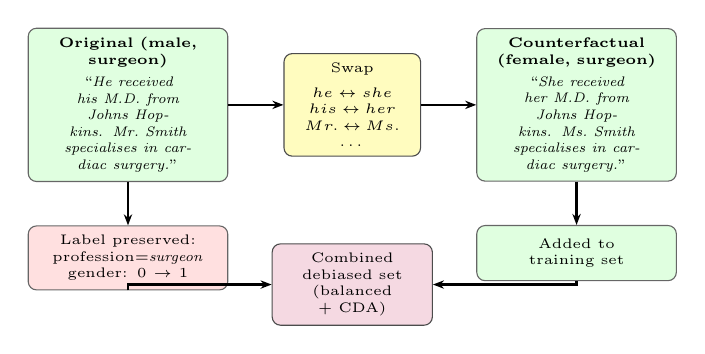
\begin{tikzpicture}[node distance=0.55cm and 0.7cm]
				\node[cdablock](orig){\textbf{Original (male, surgeon)}\\[2pt]
					\tiny``\textit{He received his M.D.\ from\\Johns Hopkins. Mr.\ Smith\\specialises in cardiac surgery.}''};
				\node[cdaswap,right=0.7cm of orig](swap){Swap\\[3pt]$he\!\leftrightarrow\!she$\\$his\!\leftrightarrow\!her$\\$Mr.\!\leftrightarrow\!Ms.$\\\ldots};
				\node[cdablock,right=0.7cm of swap](cf){\textbf{Counterfactual (female, surgeon)}\\[2pt]
					\tiny``\textit{She received her M.D.\ from\\Johns Hopkins. Ms.\ Smith\\specialises in cardiac surgery.}''};
				\draw[arrow](orig)--(swap);\draw[arrow](swap)--(cf);
				\node[cdared,below=0.55cm of orig](lorig){Label preserved:\\profession=\textit{surgeon}\\gender: $0\!\to\!1$};
				\node[cdagreen,below=0.55cm of cf](lcf){Added to\\training set};
				\draw[arrow](orig.south)--(lorig.north);\draw[arrow](cf.south)--(lcf.north);
				\node[cdacombined,below=1.1cm of swap](combined){Combined debiased set\\(balanced + CDA)};
				\draw[arrow](lorig.south)|-( combined.west);
				\draw[arrow](lcf.south)  |-(combined.east);
		\end{tikzpicture}}
		\caption{CDA: each biography is duplicated with swapped gendered surface forms.
			Profession label unchanged; gender label flipped.}
		\label{fig:cda}
	\end{figure}
	
	\subsection{Overall Results}
	The debiased model reduced the average gender gap from 26.1\% to 5.1\%.
	
	\begin{figure}[!htb]
		\centering
		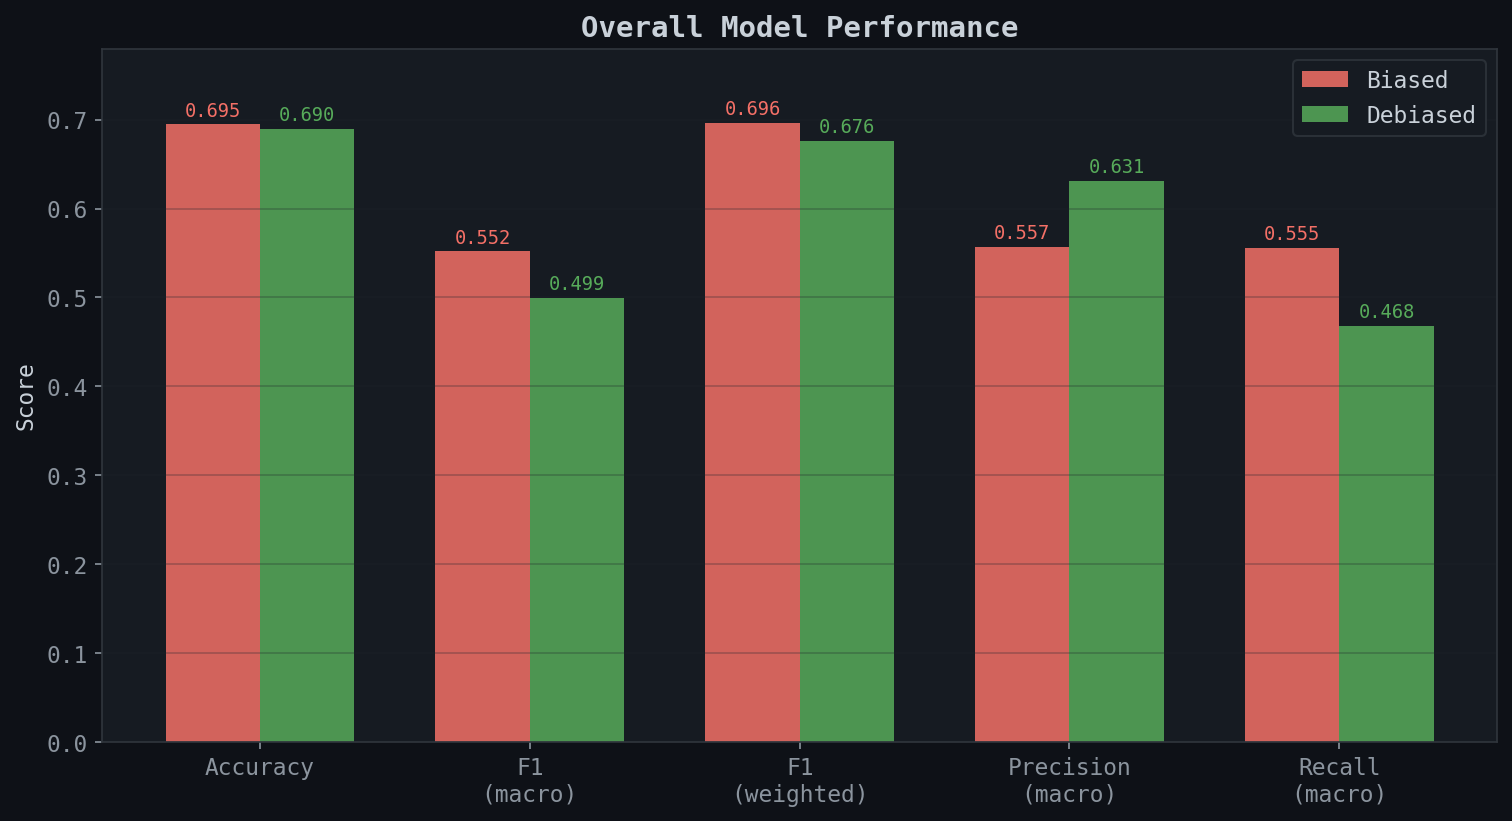
\includegraphics[width=\linewidth]{../comparison_metrics/01_overall_comparison.png}
		\caption{Summary of Accuracy, F1, and Gender Gaps.}
		\label{fig:overall_comp}
	\end{figure}
	
	\begin{figure}[!htb]
		\centering
		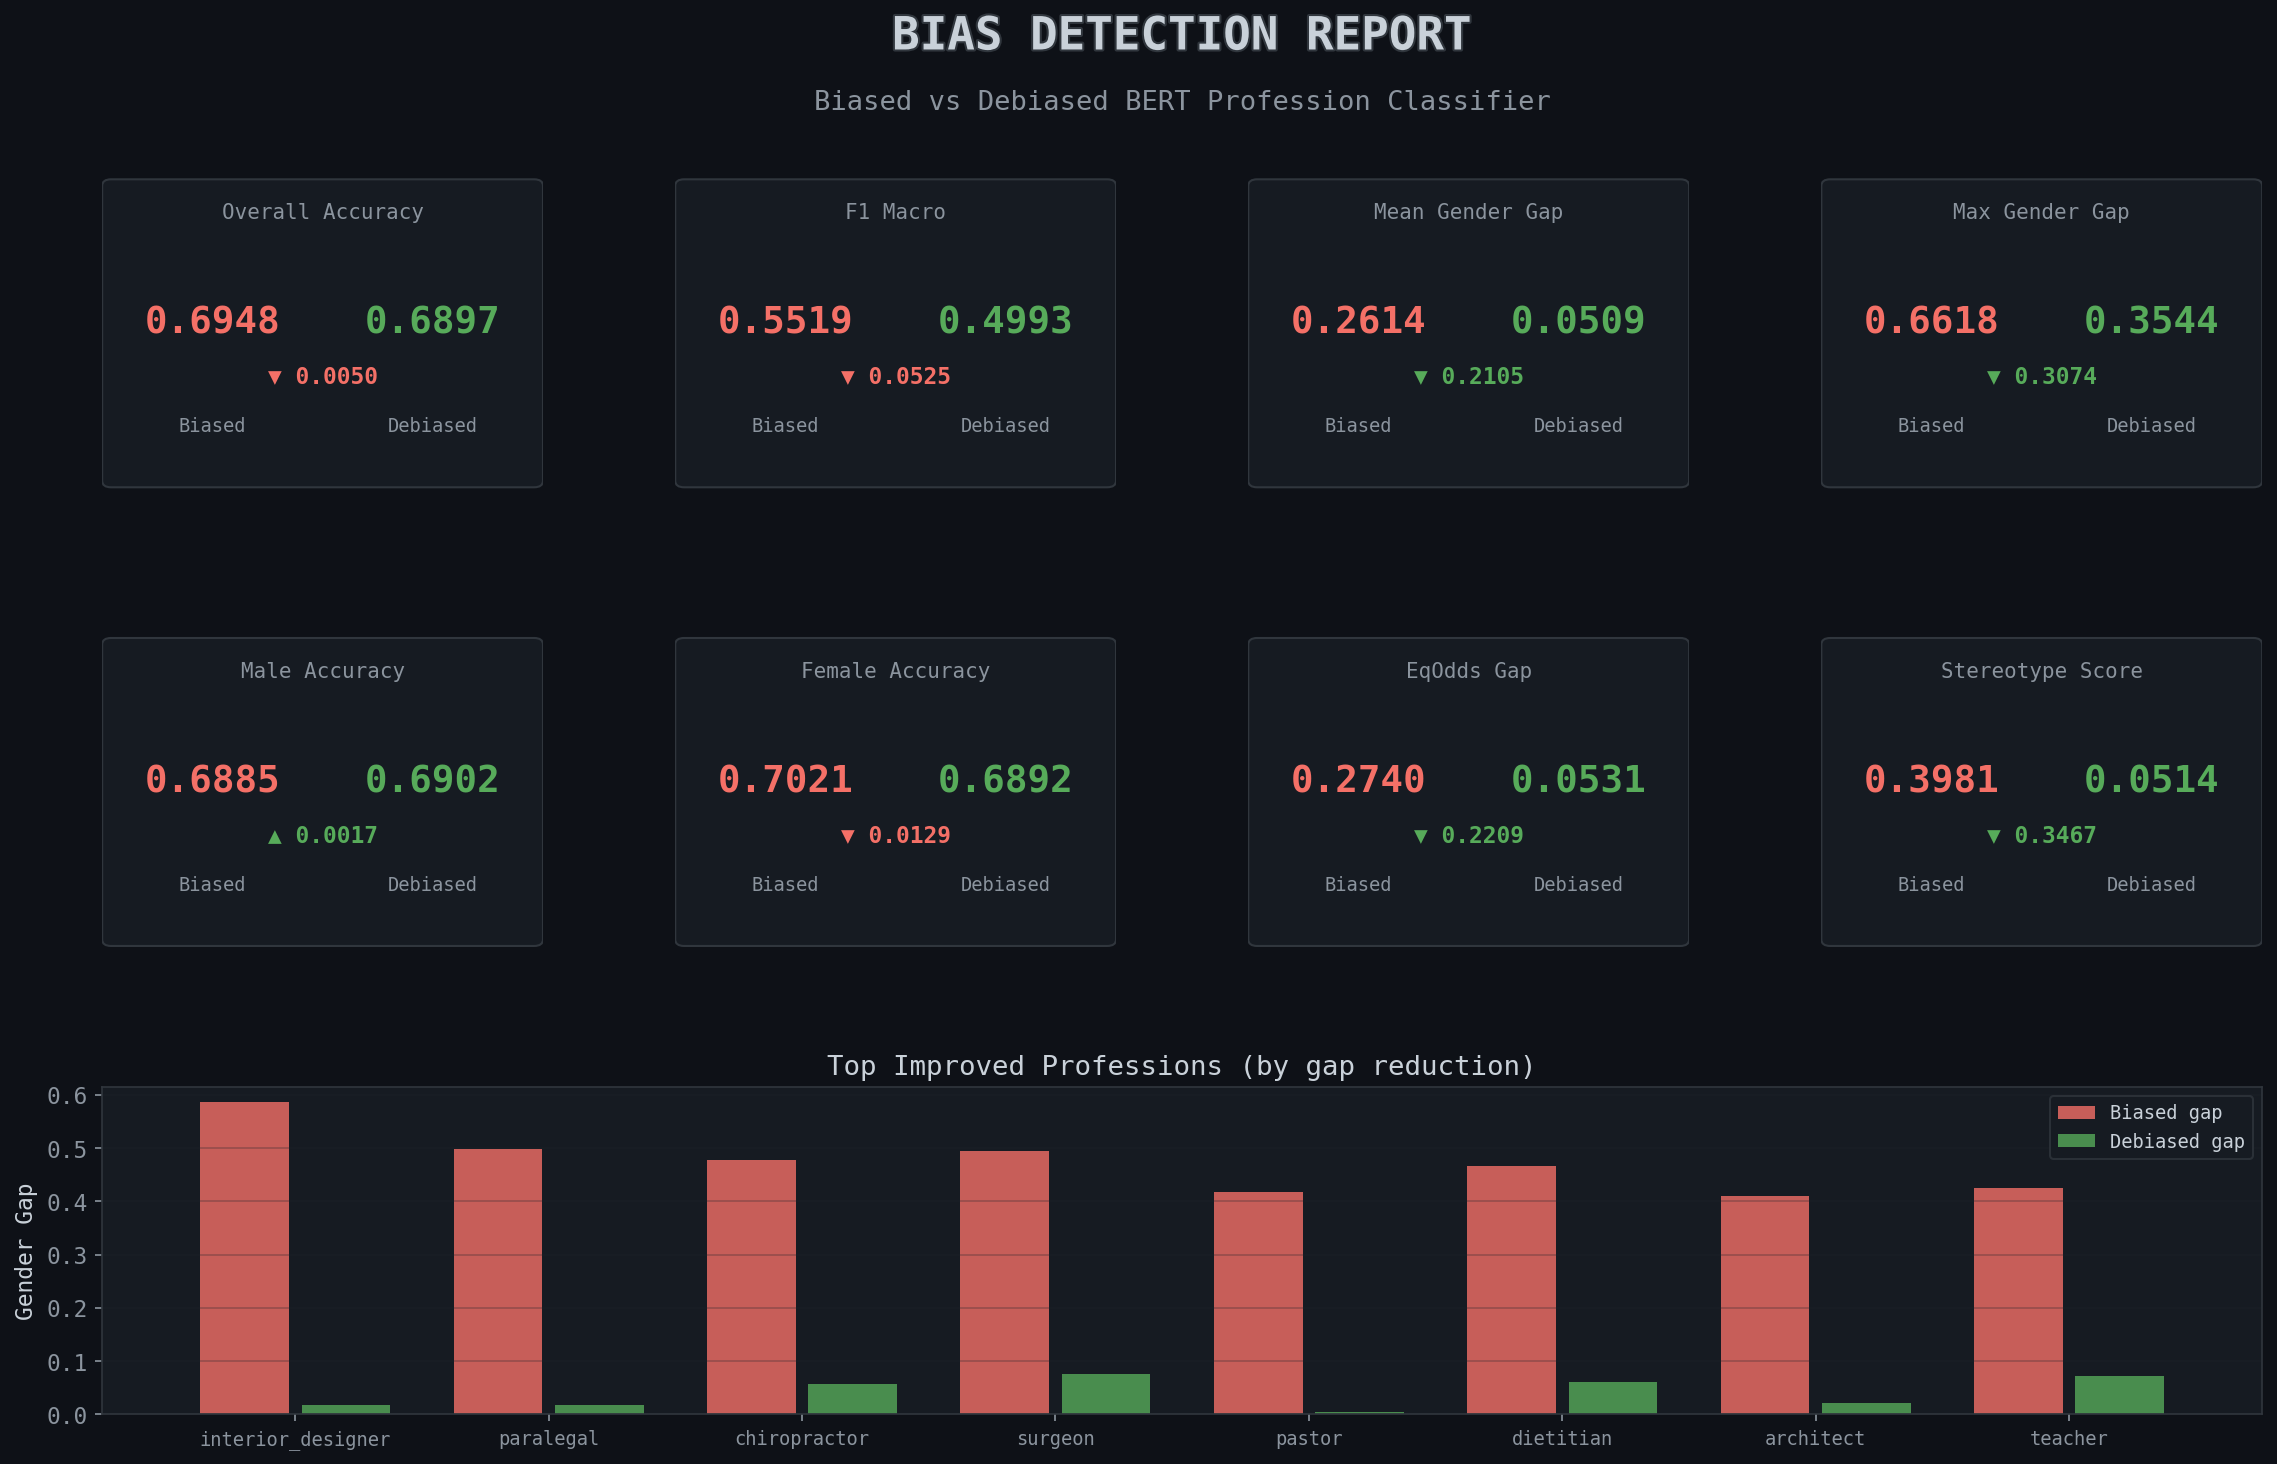
\includegraphics[width=\linewidth]{../comparison_metrics/11_summary_dashboard.png}
		\caption{Comprehensive performance dashboard.}
		\label{fig:dashboard}
	\end{figure}
	
	\subsection{Bias Metrics}
	We focused on TPR Gap, EqOdds, and Stereotype Score. The EqOdds Gap fell from 0.2740 to
	0.0531 — a 76\% improvement — ensuring equal classification probability regardless of
	gender (Figure~\ref{fig:radar}).
	
	\begin{figure}[!htb]
		\centering
		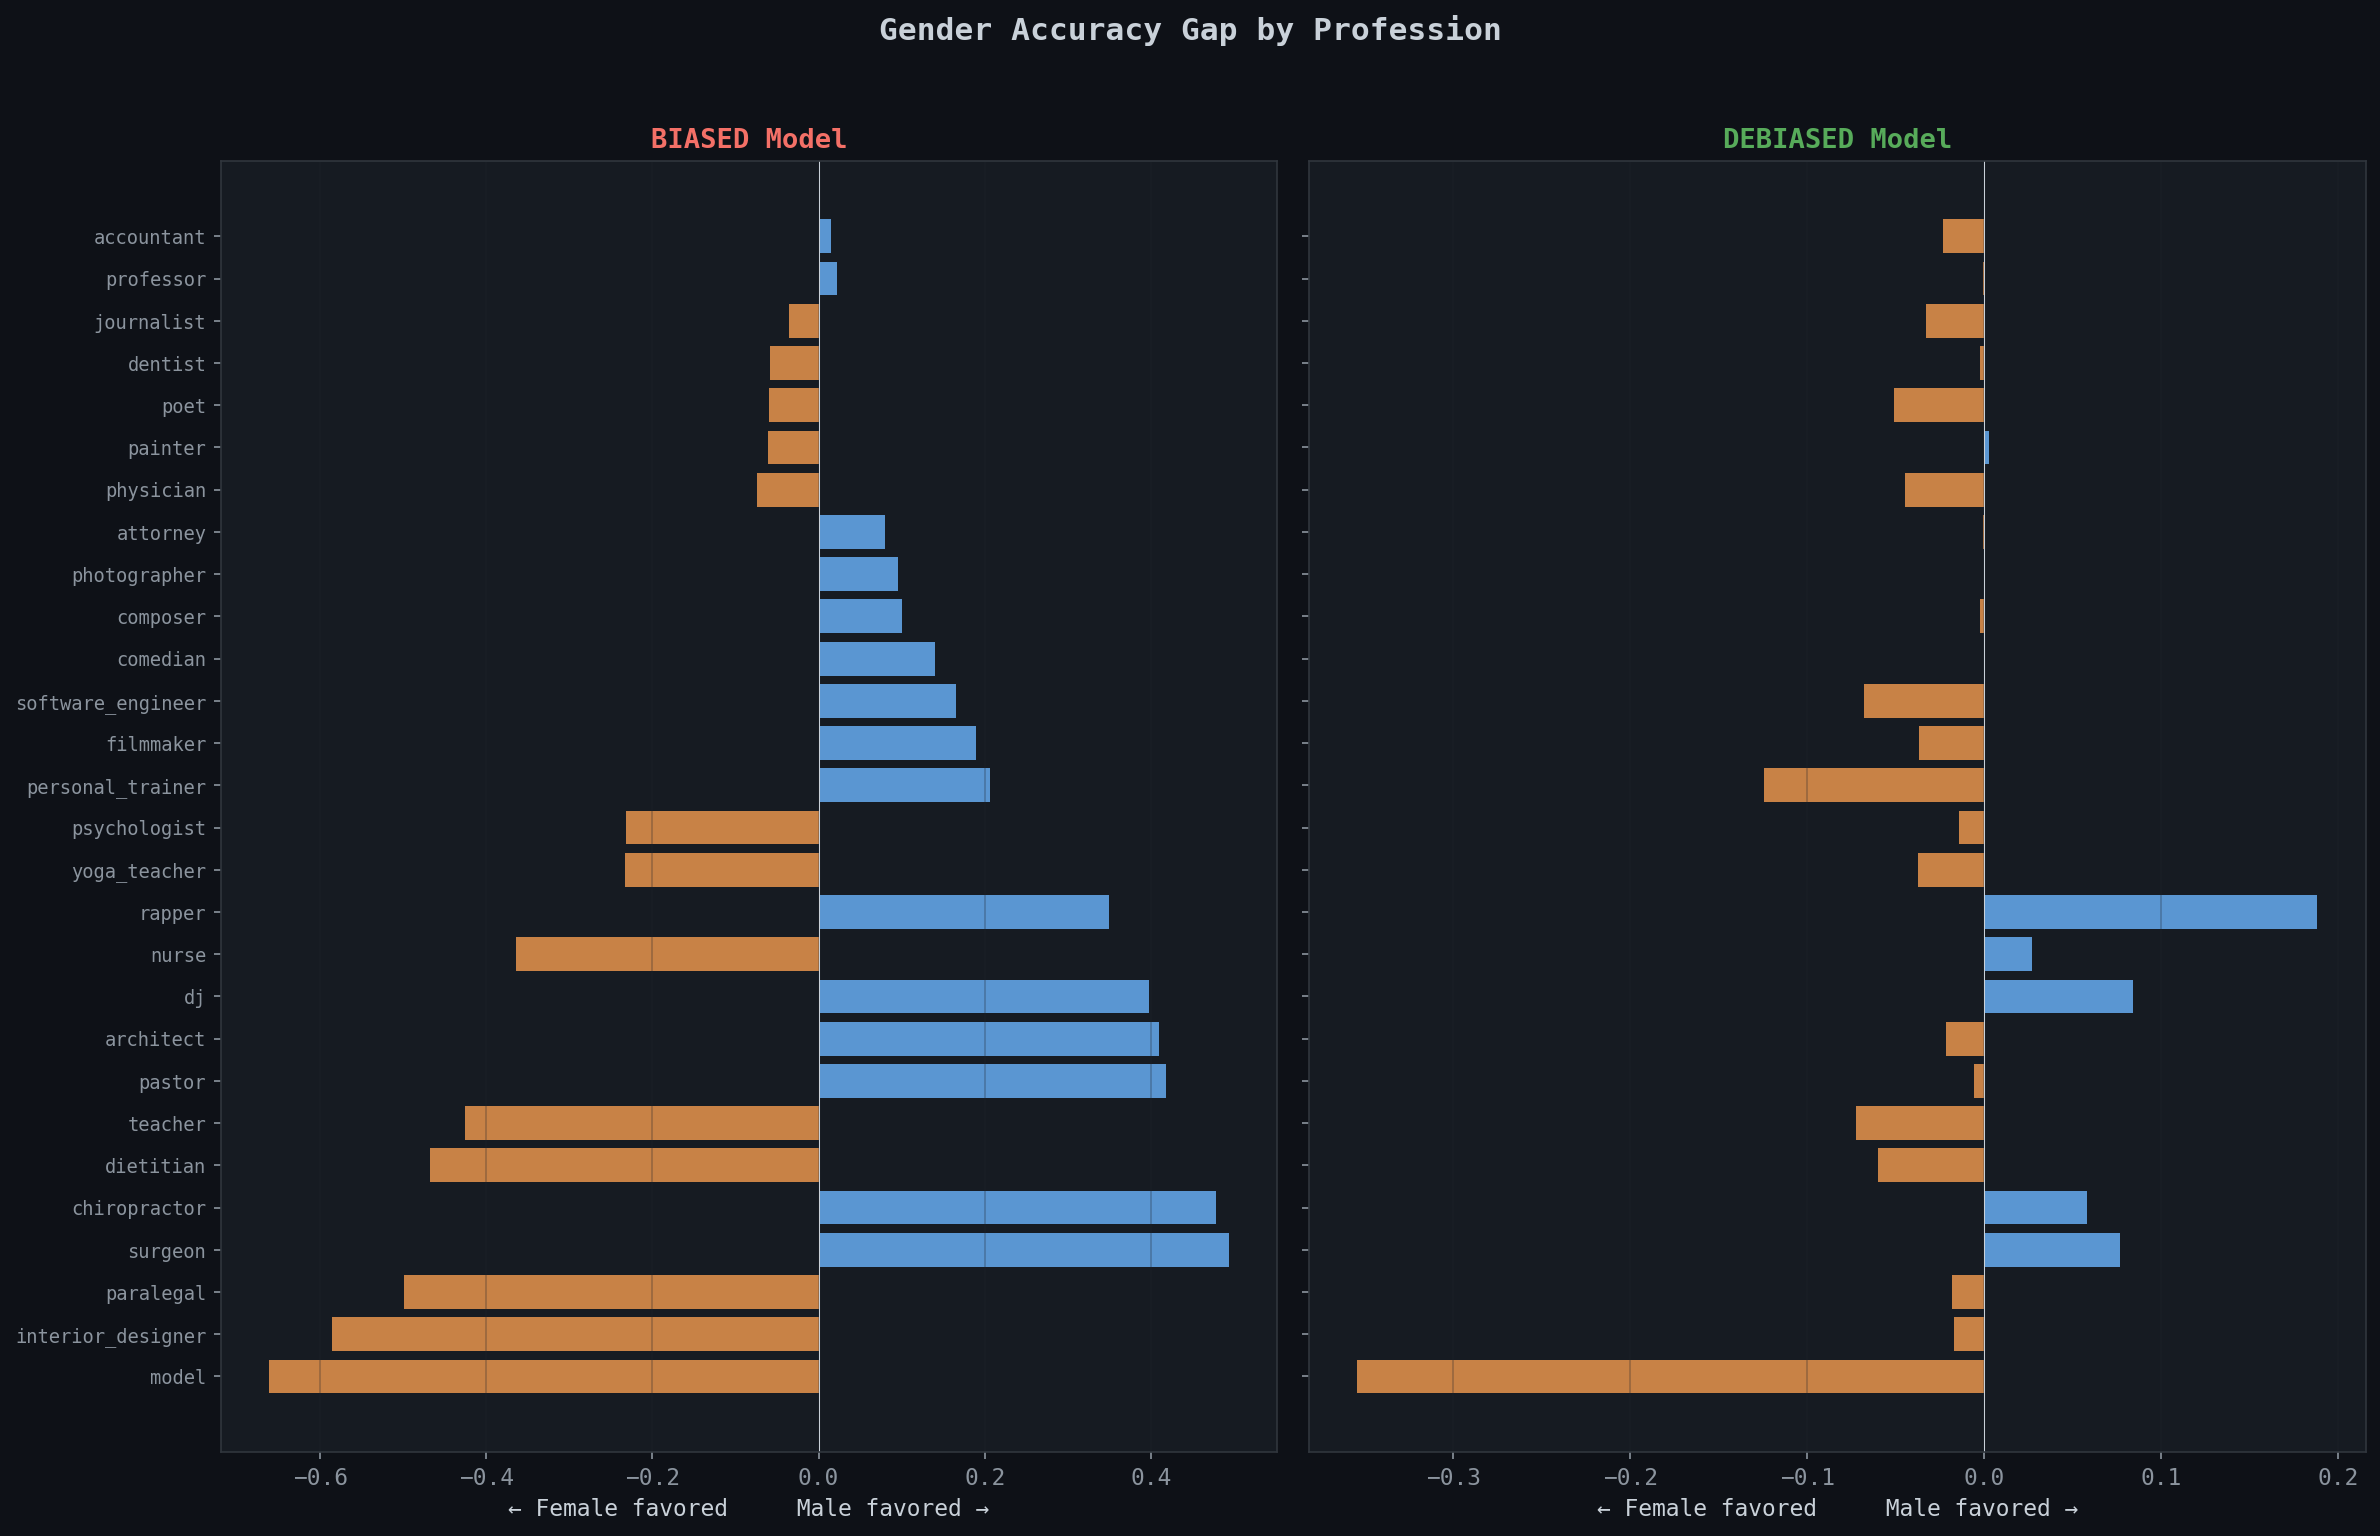
\includegraphics[width=\linewidth]{../comparison_metrics/04_gender_gap_comparison.png}
		\caption{Per-profession gender accuracy gap comparison.}
		\label{fig:gender_gap}
	\end{figure}
	
	\begin{figure}[!htb]
		\centering
		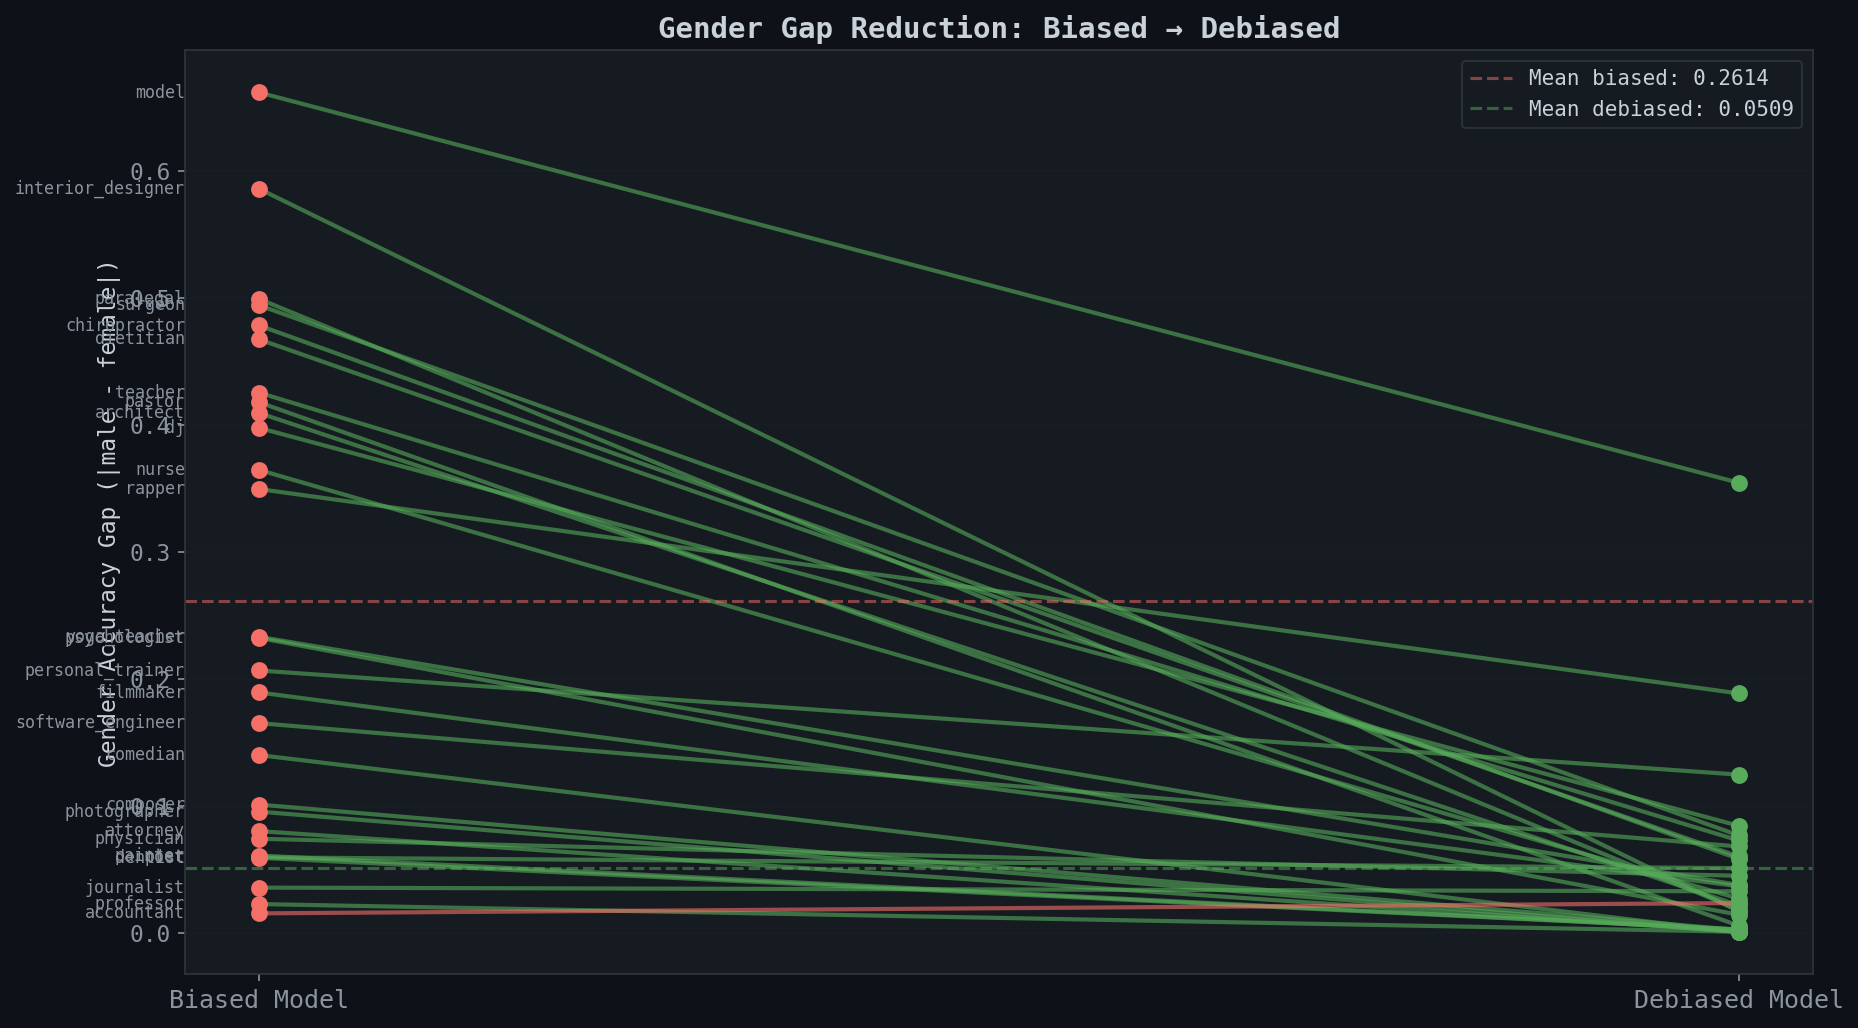
\includegraphics[width=\linewidth]{../comparison_metrics/05_gap_reduction.png}
		\caption{Reduction in bias per category: Biased $\to$ Debiased.}
		\label{fig:gap_red}
	\end{figure}
	
	\begin{figure}[!htb]
		\centering
		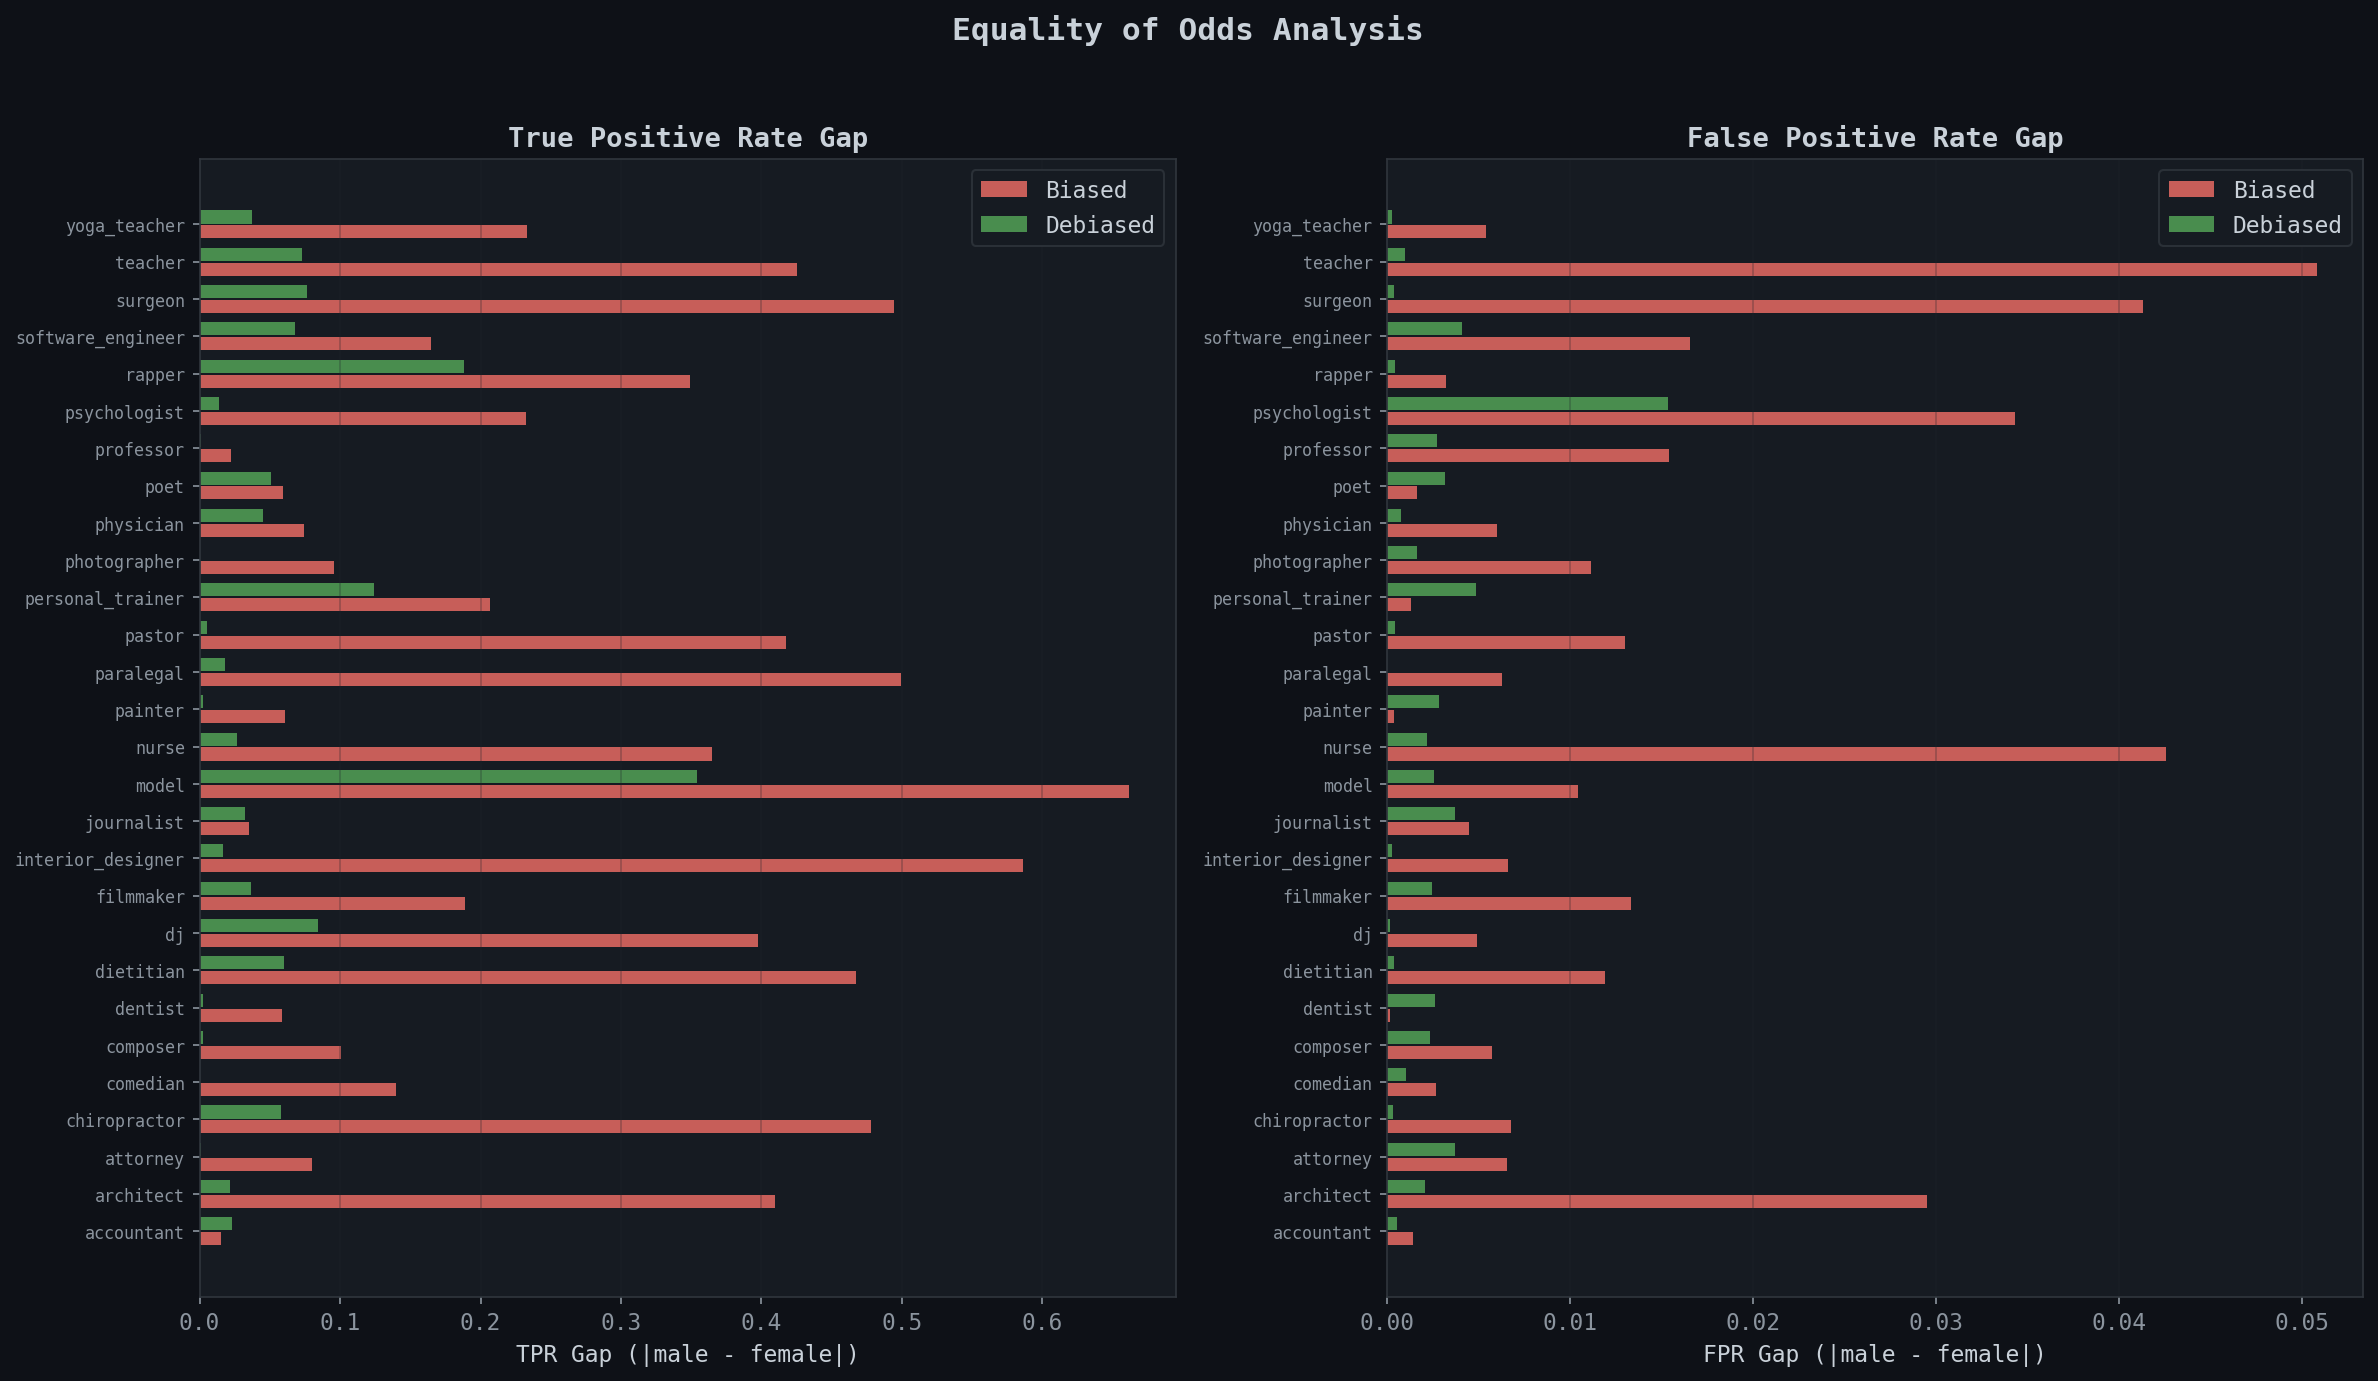
\includegraphics[width=\linewidth]{../comparison_metrics/07_tpr_fpr_gaps.png}
		\caption{True Positive Rate and False Positive Rate gaps.}
		\label{fig:tpr_fpr}
	\end{figure}
	
	\begin{figure}[!htb]
		\centering
		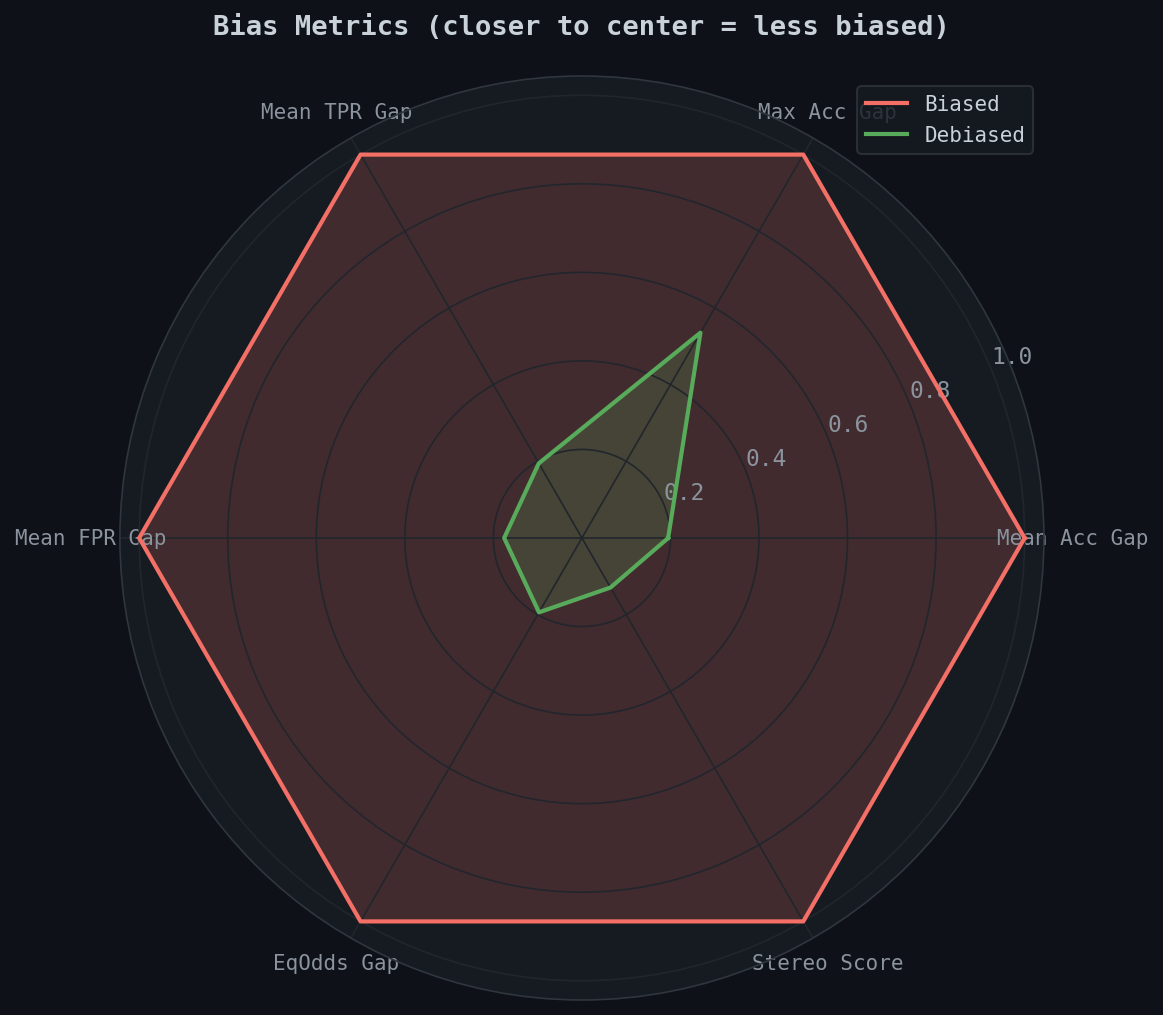
\includegraphics[width=\linewidth]{../comparison_metrics/08_bias_radar.png}
		\caption{Radar chart: biased model (red) vs.\ debiased (green) across six bias axes.}
		\label{fig:radar}
	\end{figure}
	
	\begin{figure}[!htb]
		\centering
		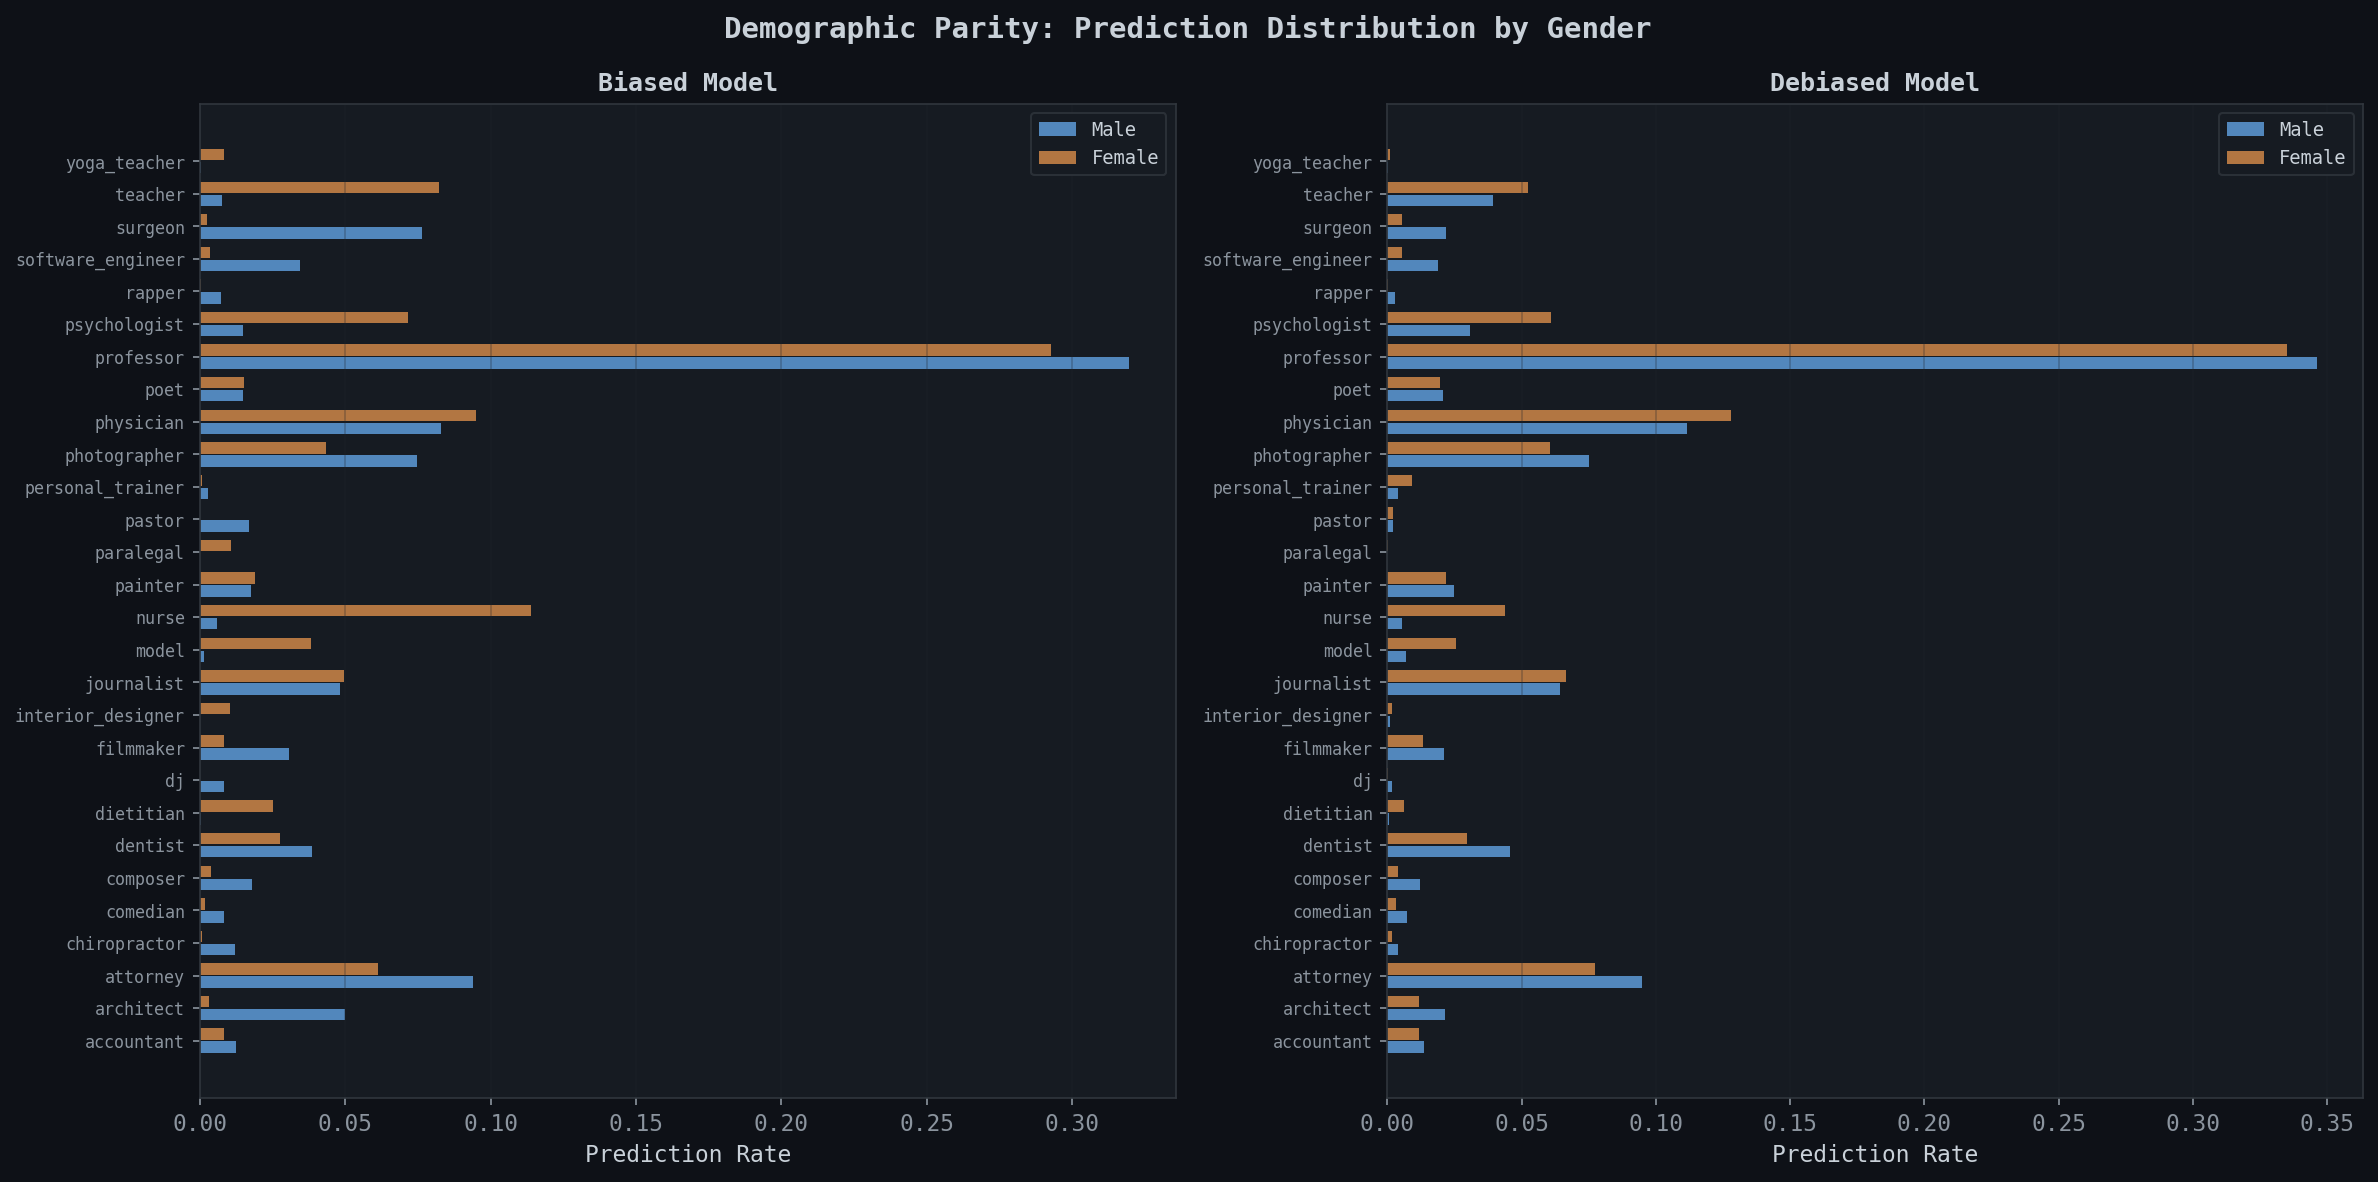
\includegraphics[width=\linewidth]{../comparison_metrics/12_demographic_parity.png}
		\caption{Demographic parity difference comparison.}
		\label{fig:dem_parity}
	\end{figure}
	
	\subsection{Performance Breakdown}
	The biased model degraded sharply on counter-stereotypical samples (e.g., female surgeons,
	male nurses), confirming it used gender as a classification shortcut. The debiased model
	achieved near-uniform accuracy across stereotypical and counter-stereotypical samples alike.
	The overall accuracy cost was negligible (69.5\%~$\to$~69.0\%) against a 26.1\%~$\to$~5.1\%
	reduction in Average Gender Gap.
	
	\begin{figure}[!htb]
		\centering
		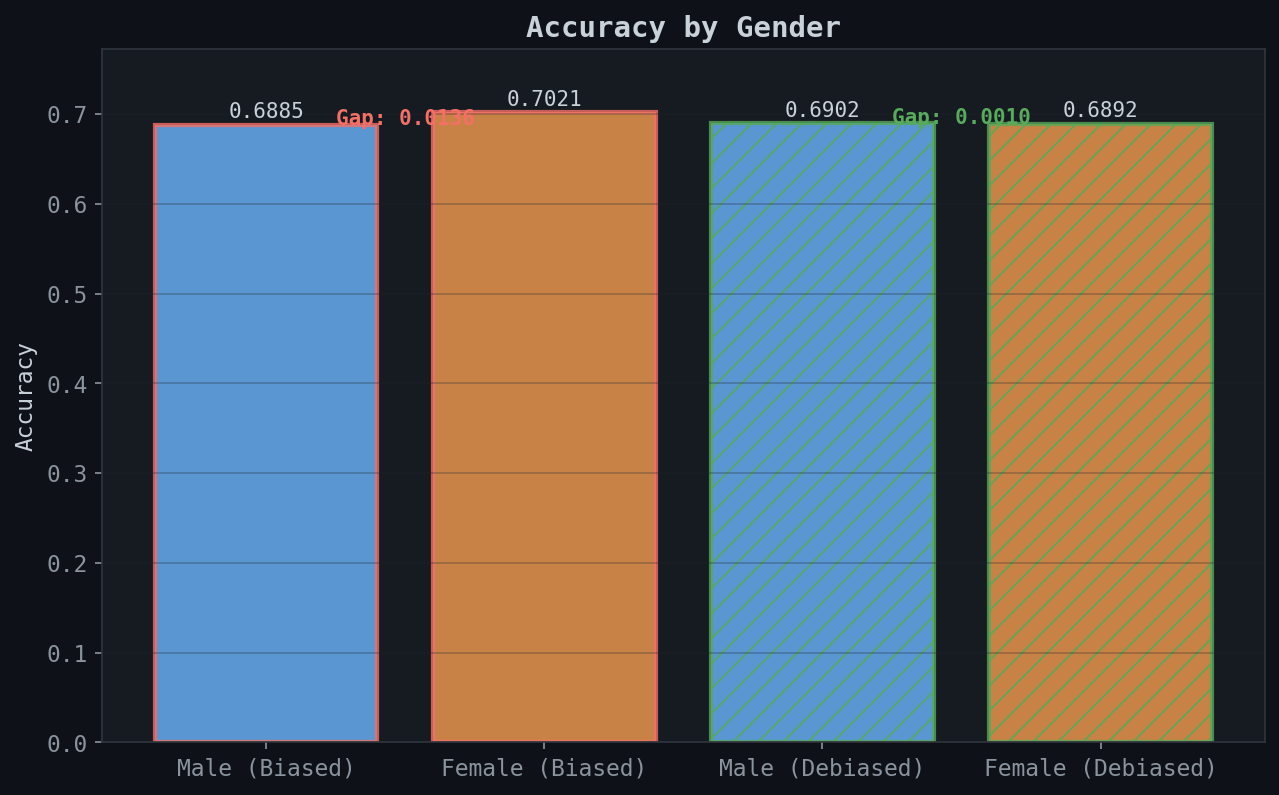
\includegraphics[width=\linewidth]{../comparison_metrics/02_gender_accuracy.png}
		\caption{Accuracy by gender: biased gap 0.0136 vs.\ debiased gap 0.0010.}
		\label{fig:gender_acc}
	\end{figure}
	
	\begin{figure}[!htb]
		\centering
		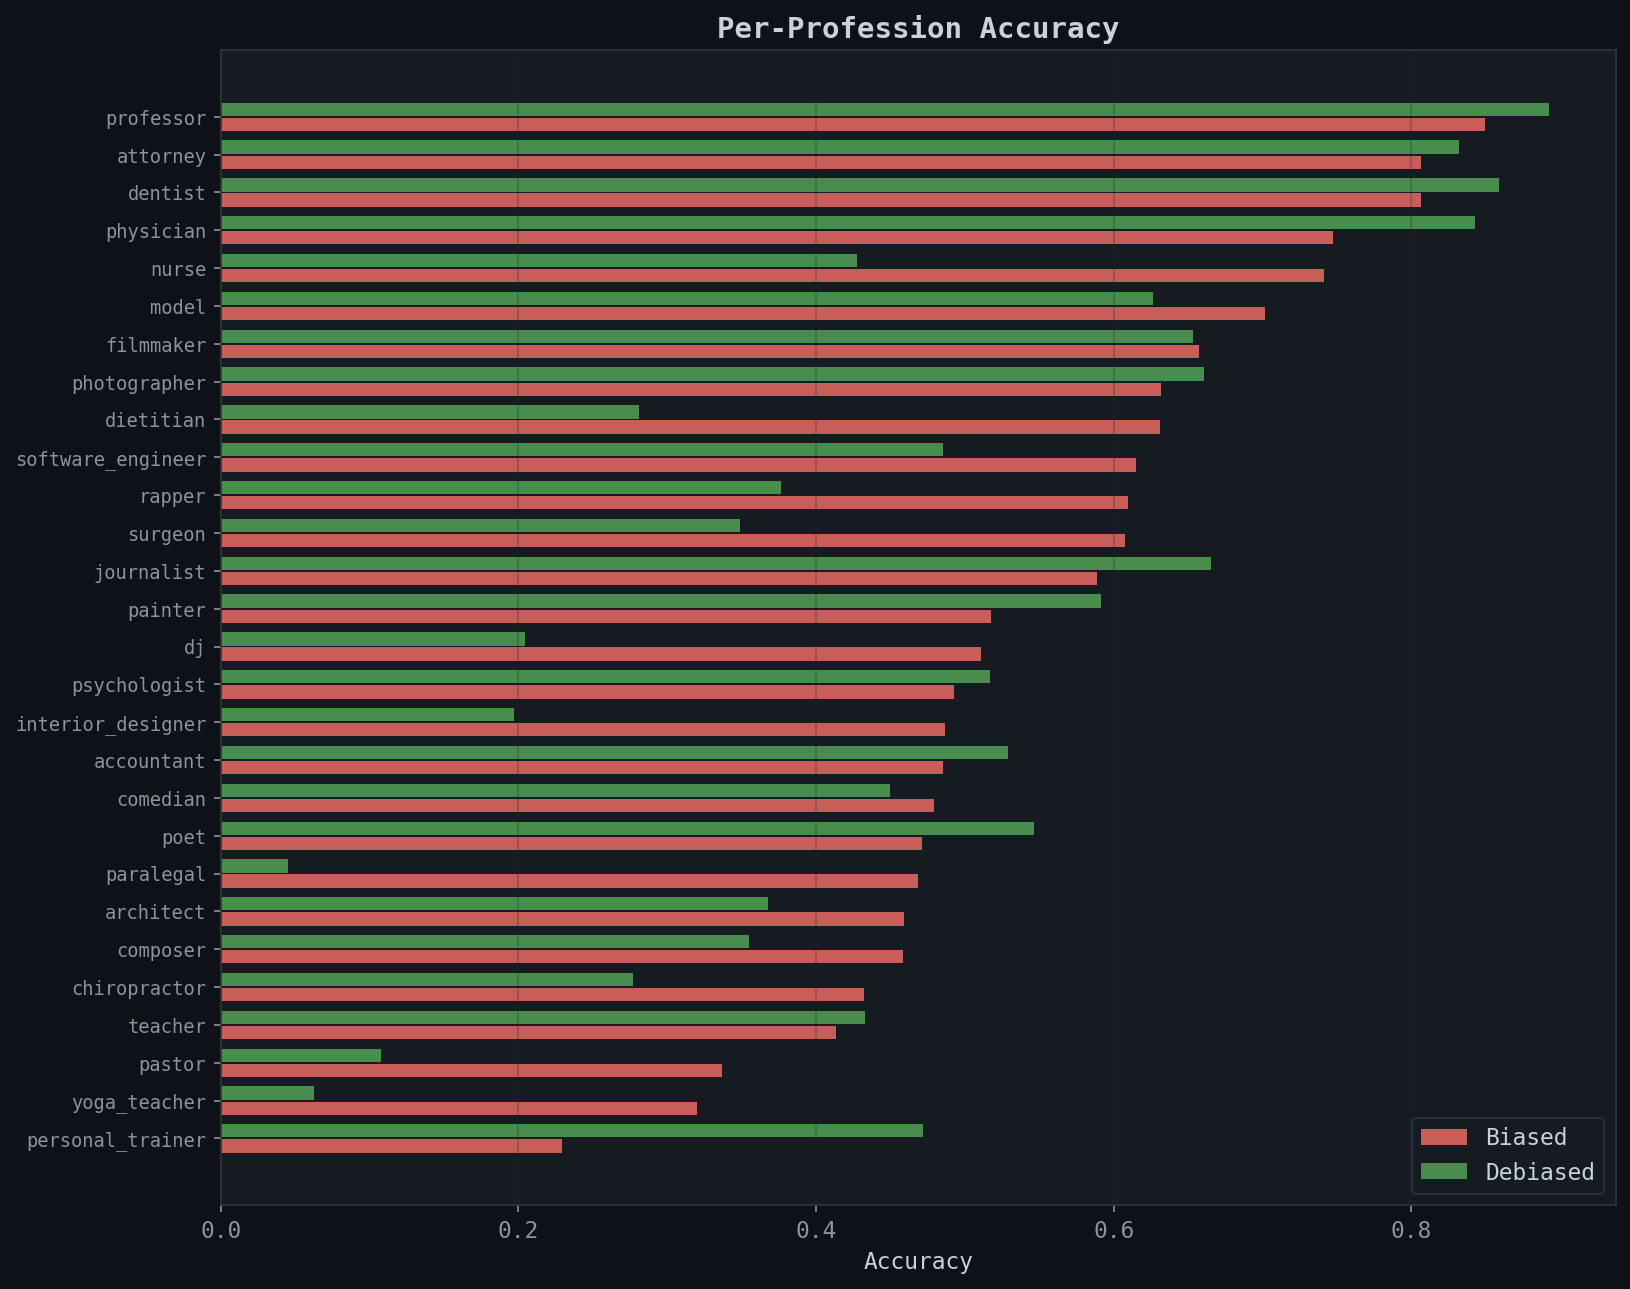
\includegraphics[width=\linewidth]{../comparison_metrics/03_per_profession_accuracy.png}
		\caption{Per-profession accuracy comparison.}
		\label{fig:per_prof}
	\end{figure}
	
	\begin{figure}[!htb]
		\centering
		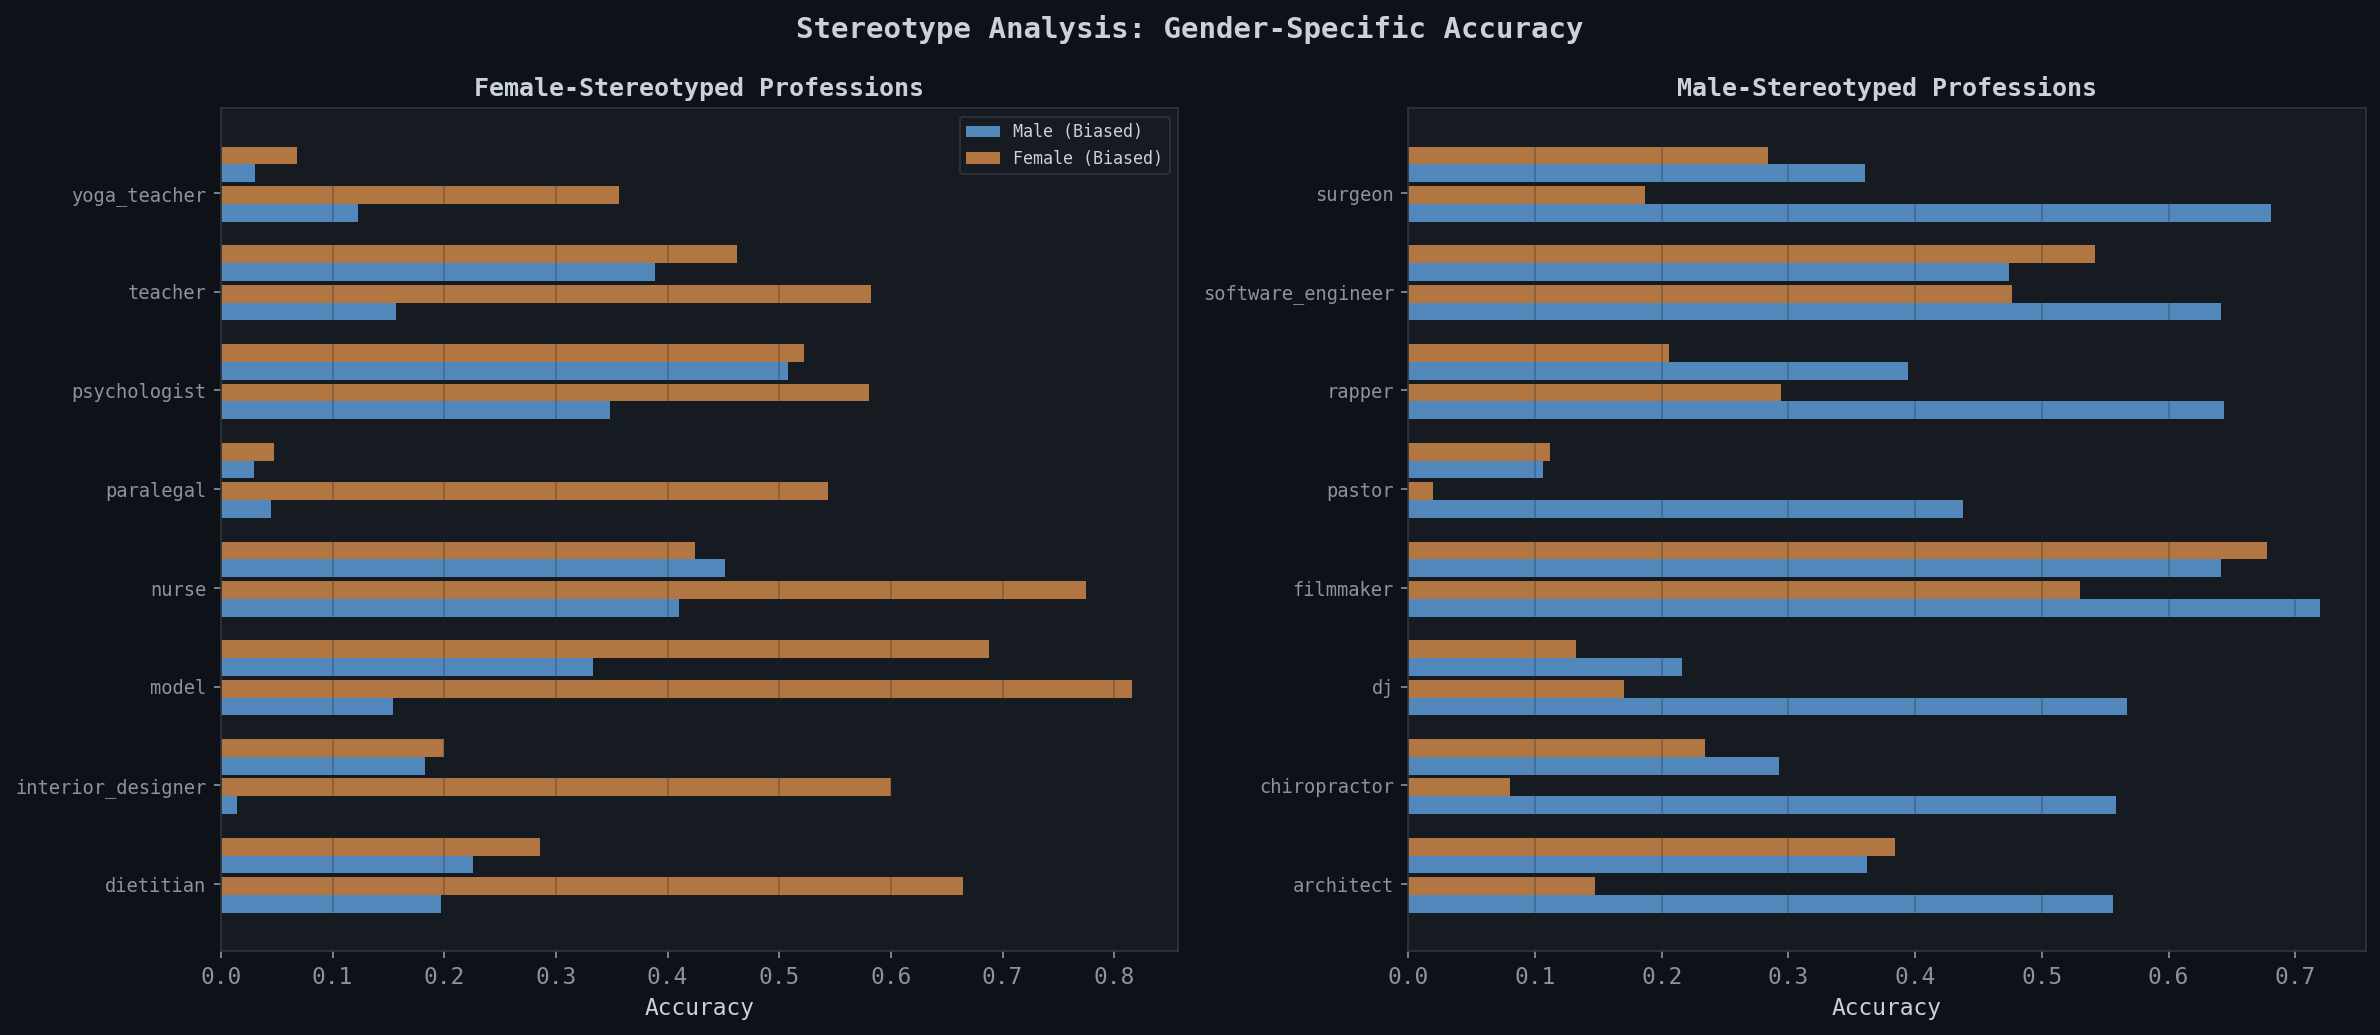
\includegraphics[width=\linewidth]{../comparison_metrics/09_stereotype_analysis.png}
		\caption{Accuracy on Stereotypical vs.\ Counter-Stereotypical samples.}
		\label{fig:stereo}
	\end{figure}
	
	\begin{figure}[!htb]
		\centering
		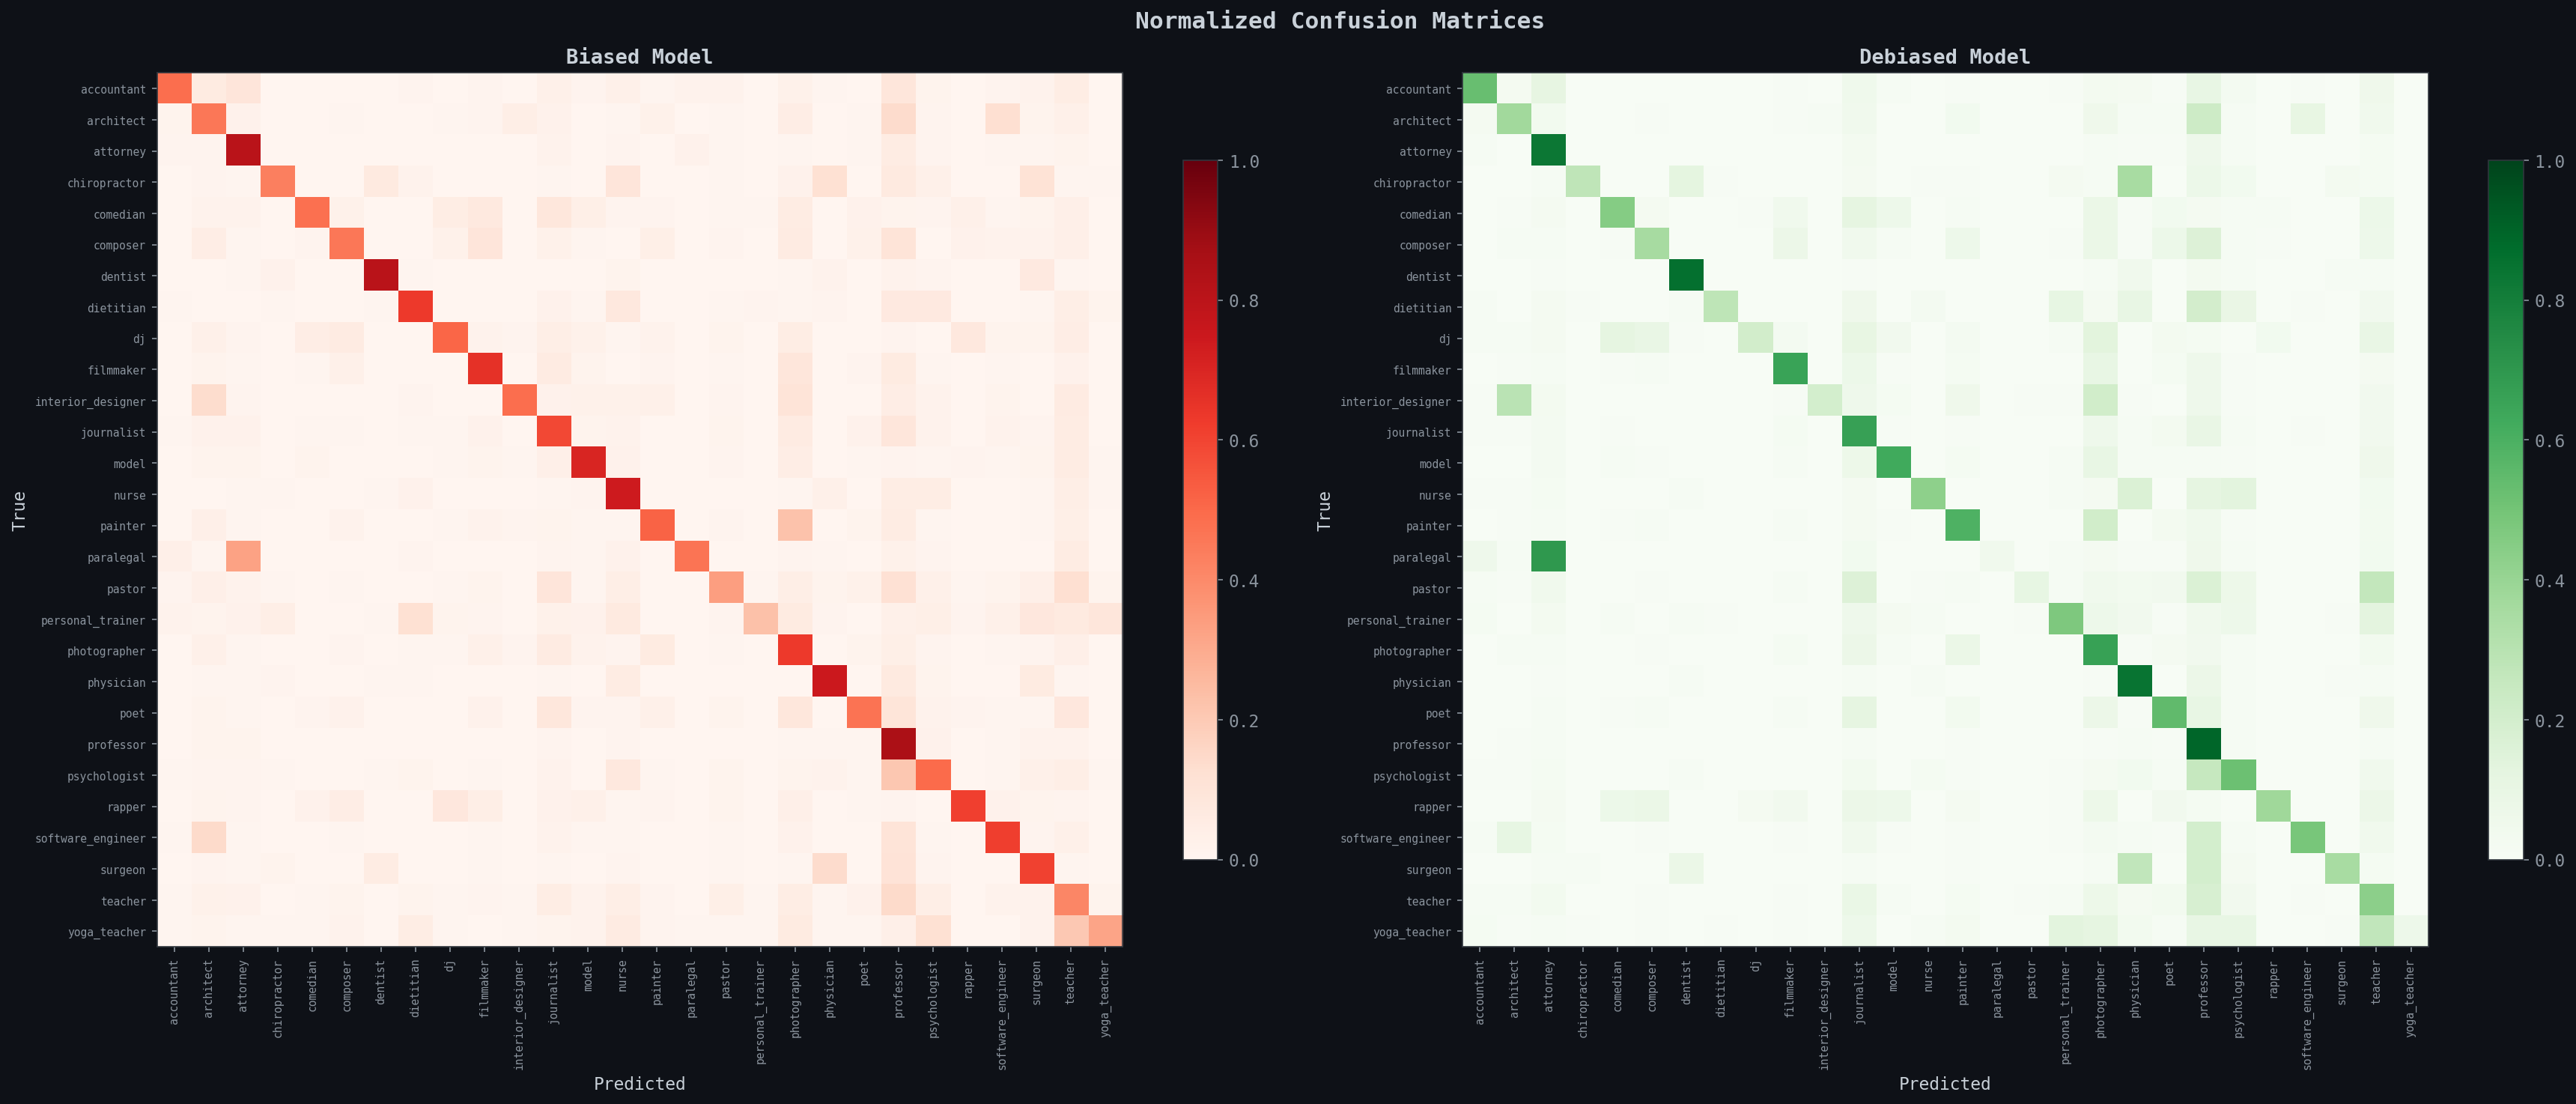
\includegraphics[width=\linewidth]{../comparison_metrics/06_confusion_matrices.png}
		\caption{Normalized confusion matrices for both models.}
		\label{fig:confusion}
	\end{figure}
	
	\begin{figure}[!htb]
		\centering
		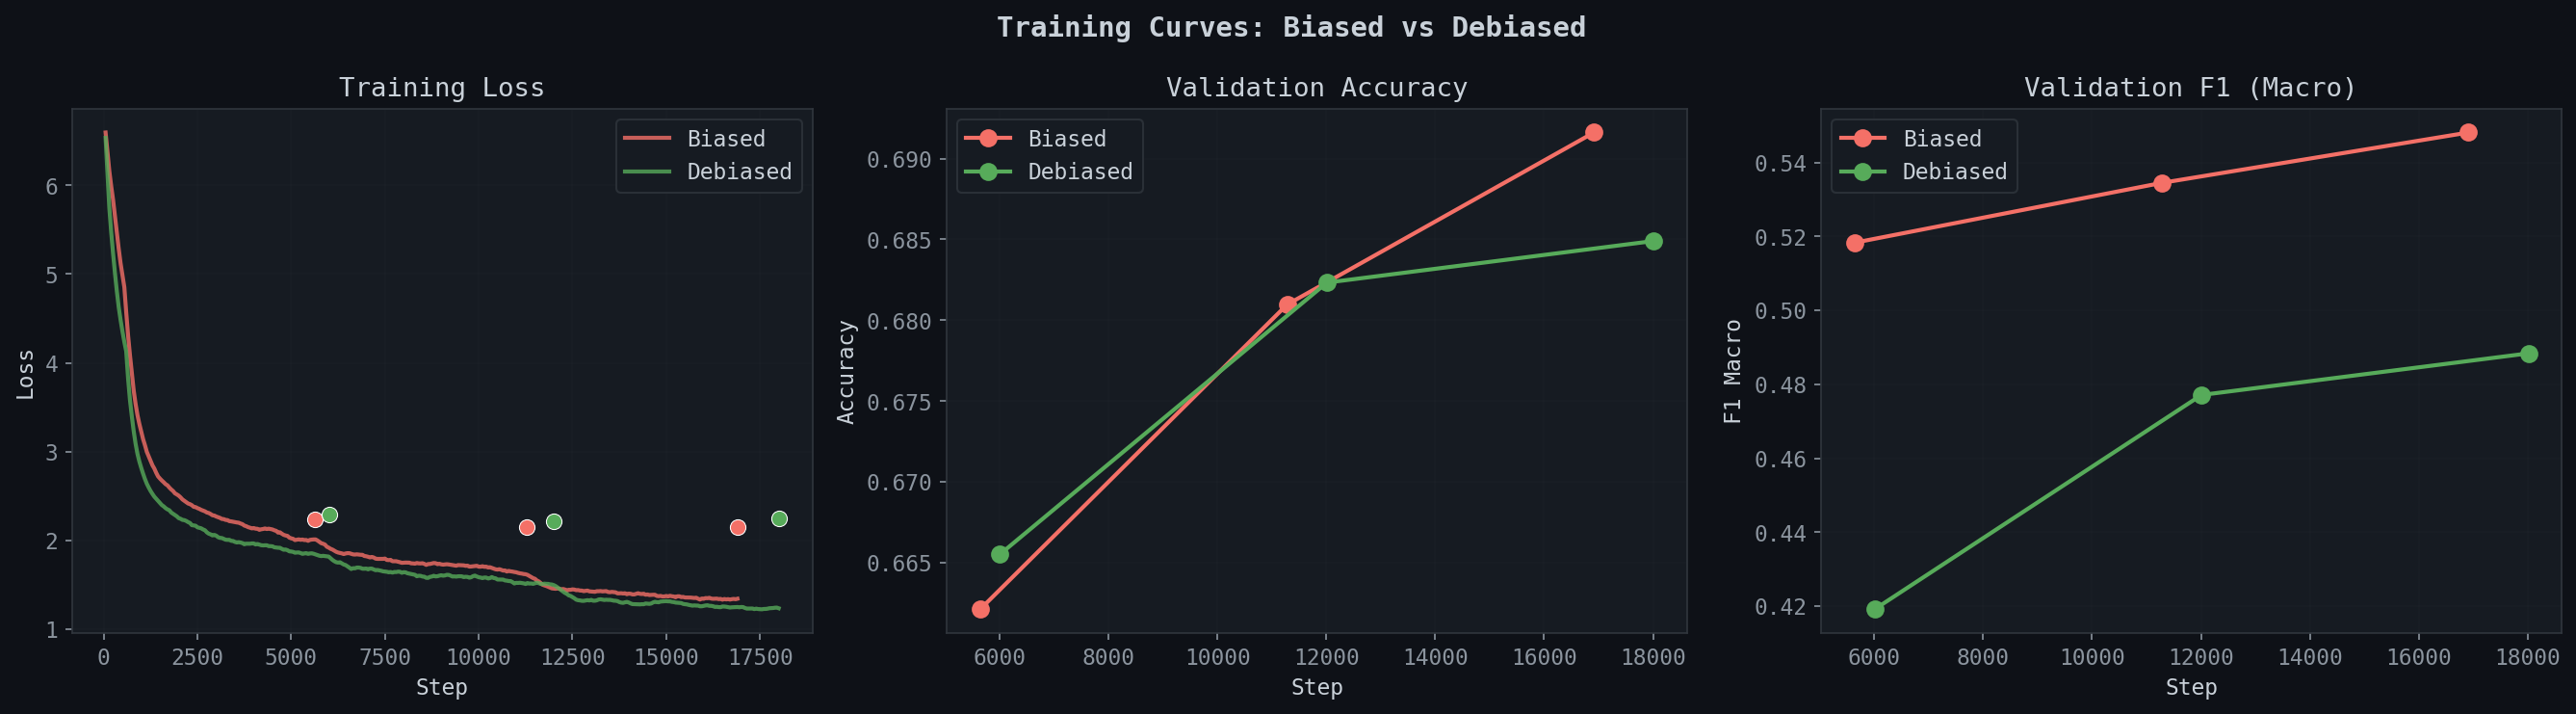
\includegraphics[width=\linewidth]{../comparison_metrics/10_training_curves.png}
		\caption{Fine-tuning training curves: loss, validation accuracy, F1 macro.}
		\label{fig:training_curves}
	\end{figure}
	
	% ======================================================================
	\section{Conclusion}
	% ======================================================================
	Across all 30 metrics, counterfactual data augmentation significantly improves model
	fairness without substantial loss in predictive power. LLM-based pipelines inherit
	systemic biases from datasets like Bias-in-Bios, where professions such as ``Dietitian''
	and ``Nurse'' are heavily female-skewed while ``Surgeon'' and ``Software Engineer''
	remain male-dominated. By balancing the training distribution via CDA, we successfully
	decoupled gender indicators from professional labels, achieving a 76\% reduction in
	EqOdds Gap at negligible cost to overall classification accuracy.
	
\end{document}